% Chapter Template

\chapter{Billiards and quantum chaos} % Main chapter title

\label{Chapter05} % Change X to a consecutive number; for referencing this chapter elsewhere, use \ref{ChapterX}
\thispagestyle{empty}
%----------------------------------------------------------------------------------------
%	SECTION 1
%----------------------------------------------------------------------------------------

\section{Introduction}
\label{sec:intro}
%\addcontentsline{toc}{section}{Main Section 1}%\nameref{sec:intro}}

%\textsf{E' questo il font}?

The main \virg{physical} dynamical system we will consider in this thesis is a billiard, which is a model where a (usually dimensionless) particle moves within a bounded domain in the Euclidian space $\R^{n}$ and bounces off the boundary of the domain elastically. Physically this can be interpreted in several different ways. But we will also consider the same kind of motion but on surfaces, which will have negative curvature, for reasons that we will learn more about later.\\

The bouncing billiard can be realized, from a physical point of view, by considering, for example, a potential function which zero inside of the considered domain, and equal to infinity otherwise. However, regardless of their physical realization, these kind of system can exhibit a number of interesting properties.

More formally, we will consider the following definition.

\begin{defin}
A \emph{dynamical metric system} is the quadruple $(X,\chi,\mu,R)$ where $(X,\chi,\mu)$ is a metric space with $\sigma$-algebra $\chi$ and $R$ is a $\mu$-measurable map such that $\mu$ is $R$-invariant, i.e. $R_{\ast}\mu=\mu$. 
\end{defin}

Often, $R$ will be more regular than just being measurable. We are now ready to introduce the concept of billiard systems. We will consider essentially, as already mentioned, two main cases:
\begin{itemize}
\item \boldsf{Billiard flows}:\\
A \emph{billiard} is a bounded, planar domain $\Omega$ with a piecewise smooth boundary. The billiard flow is the classical frictionless motion of a particle inside $\Omega$, with angle of incidence to the boundary $\partial\Omega$ equal to angle of reflection off $\partial\Omega$; the total kinetic energy is preserved. In this case, the preserved measure is a multiple of Lebesgue measure, i.e. Liouville measure, given explicity by $\mu_{L}=\frac{\one_{\Omega}}{\lambda(\Omega)}$, where $\lambda(\Omega)$ is the measure of set $\Omega$. If we consider the unit tangent space $T^{1}\Omega$, then the Liouville measure is given by $\mu_{L}=\frac{\one_{\Omega}}{2\pi\lambda(\Omega)}$. 
\item \boldsf{Geodesic flows (on manifolds)}:\\
If $M$ is a Riemannian manifold with metric $g$, then for each point $q\in M$, there is one and only one \emph{geodesic} (i.e. path of minimal length) given a unit direction. So the classical frictionless motion of a particle along local geodesics gives the desired flow. Moreover, it's well defined the unit tangent space $T^{1}M$ and in this case the Liouville measure is given by $\mu_{L}=\frac{\one}{2\pi\lambda(M)}$ where $\lambda(M)$ is the \virg{area} of $M$, with respect to metric $g$. 
\end{itemize}
In both cases, we will denote the considered flow with $\Phi_{t}$. Sometimes, it is more convenient to consider only a \emph{discretization} of the flow; for example, in billiard flow case, it can be helpful to consider the map $\Psi=\Phi_{T}^{n}$ which gives the position of a point $q\in\Omega$ after time $nT$.\\
Billiards systems, even if simple in their definition, can exhibit a certain degree of \emph{chaotical properties}. A good property to look at for this type of features is ergodicity.

\begin{nteo}[Ergodicity, discrete case]
\label{definteo:ergodic_discrete}
Let $(X,\chi,\mu,R)$ be a dynamical metric system, with $X$ of finite measure, i.e. a probability space. The followings hold and give a definition of a (discrete) ergodic system:
\begin{compactitem}
\item if $B$ is $R$-invariant, then $\mu(B)=0$ or $\mu(B^{\compl})=0$
\item if $\mu(A),\mu(B)>0$ for measurable sets $A,B$, then it does exist a $k\geq0$ such that $\mu(A\cap R^{-k}[B])>0$.
\end{compactitem}
\end{nteo}

Roughly speaking, ergodicity requires that a dynamical system cannot be decomposed in smaller and indipendent dynamical system and every set is taken across all the space $X$ through the action of map $R^{-k}$, with $k\geq0$. Moreover, every subset $A$ must be \virg{mixed} with every other subset $B$, in a certain proportion. In fact, another important feature is the concept of \emph{mixing}. 

\begin{defin}[Mixing]
\label{defin:mixing_discrete}
A dynamical metric system $(X,\chi,\mu,R)$ is called \emph{mixing} if $\,\forall A,B\in\chi$ we have
\[
\lim_{n\to\infty}\abs{\mu(A\cap R^{-n}[B])-\mu(A)\mu(B)}=0.
\]
\end{defin}

Mixing is indeed a \underline{stronger property} than ergodicity, because it does not only require that the system mixes itself, but every couple of sets $A,B$ should be mixed in \emph{the right proportion}.\\
We can rewrite these definition for the continuos case.

\begin{defin}[Ergodicity and mixing, continuos case]
\label{defin:ergodic_mixing_contin}
Let $(X,\chi,\mu,\Phi_{t})$ be a dynamical metric system, with $X$ of finite measure, i.e. a probability space.
\begin{compactitem}
\item The flow $\Phi_{t}$ is \emph{ergodic} if for every measurable set $B\subset X$ which is $R_{t}$ invariant for every $t$, then $\mu(B)=0$ or $\mu(B^{\compl})=0$;
\item The flow $\Phi_{t}$ is \emph{mixing} if for every measurable sets $A,B\subset X$
\[
\mu(A\cap\Phi_{t}^{-1}[B])\stackrel{t\to\infty}{\longrightarrow}\mu(A)\mu(B).
\]
\end{compactitem}
\end{defin}

A more pictorial way to understand ergodicity from a physical point of view is given by the following result, due to Birkhoff.

\begin{nteo}[Birkhoff]
\label{teo:birkhoff}
The flow $\Phi_{t}$ is ergodic iff $\forall f\in L^{1}(X)$,
\[
\lim_{T\to\infty}\frac{1}{T}\int_{0}^{T}f\circ\Phi_{t}(x)\dd t = \int_{X}\vphi \dd\mu
\]
for $\mu$-a.e. $x\in X$.
\end{nteo}

What theorem \ref{teo:birkhoff} states is that, in an ergodic system, the trajectories are equidistributed in the phase space. There is also a reinterpretation of ergodicity from a \virg{spectral} point of view, considering the precomposing map $R^{\ast}f=f\circ R$.

\begin{nteo}
\label{teo:ergodic_spectral} 
Let $(X,\chi,\mu,R)$ be a metric system e let $p\in[1,+\infty]$. The followings are equivalent:
\begin{compactitem}
\item the system $(X,\chi,\mu,R)$ is ergodic;
\item the eigenspace of $R^{\ast}$ in $L_{p}$ corrispondent to eigenvalue $1$ is made up only by a.e. constant functions $\mathbb{C}\one$.
\end{compactitem}
\end{nteo}

We will go deeper into this \virg{spectral} approach in the following chapters.


\subsection{Examples}

We are now ready to analyze some examples. At first, we will consider some classical billiards.\\[2mm]

\noindent{\large \boldsf{Billiards}}:

\begin{nese}[Biliardo circolare, ellittico]
The circular, elliptic billiard is given by the classical \virg{bouncing motion} and a domain $\Omega\subset\R^{2}$ which is given by a circle or, more generally, an ellipse. In this case, the billiard \underline{is not ergodic}, as it can be easy seen in the circular case. In fact, if the angle of first bounce is $\vtheta$, then for the symmetry of the circle, this angle is constant through every bounce and so it is a constant quantity over an orbit and depending on the considered orbit. So, for theorem \ref{teo:ergodic_spectral}, this system cannot be ergodic. This property has a concrete impact on the aspect of a generic orbit. Seeing figure \ref{fig:ell_circ_billiards}, it can be observed that a generic orbit avoids whole parts of the domain.  
\end{nese}


\begin{figure}[H]
\centering
  \begin{subfigure}[b]{0.3\textwidth}
  \centering
    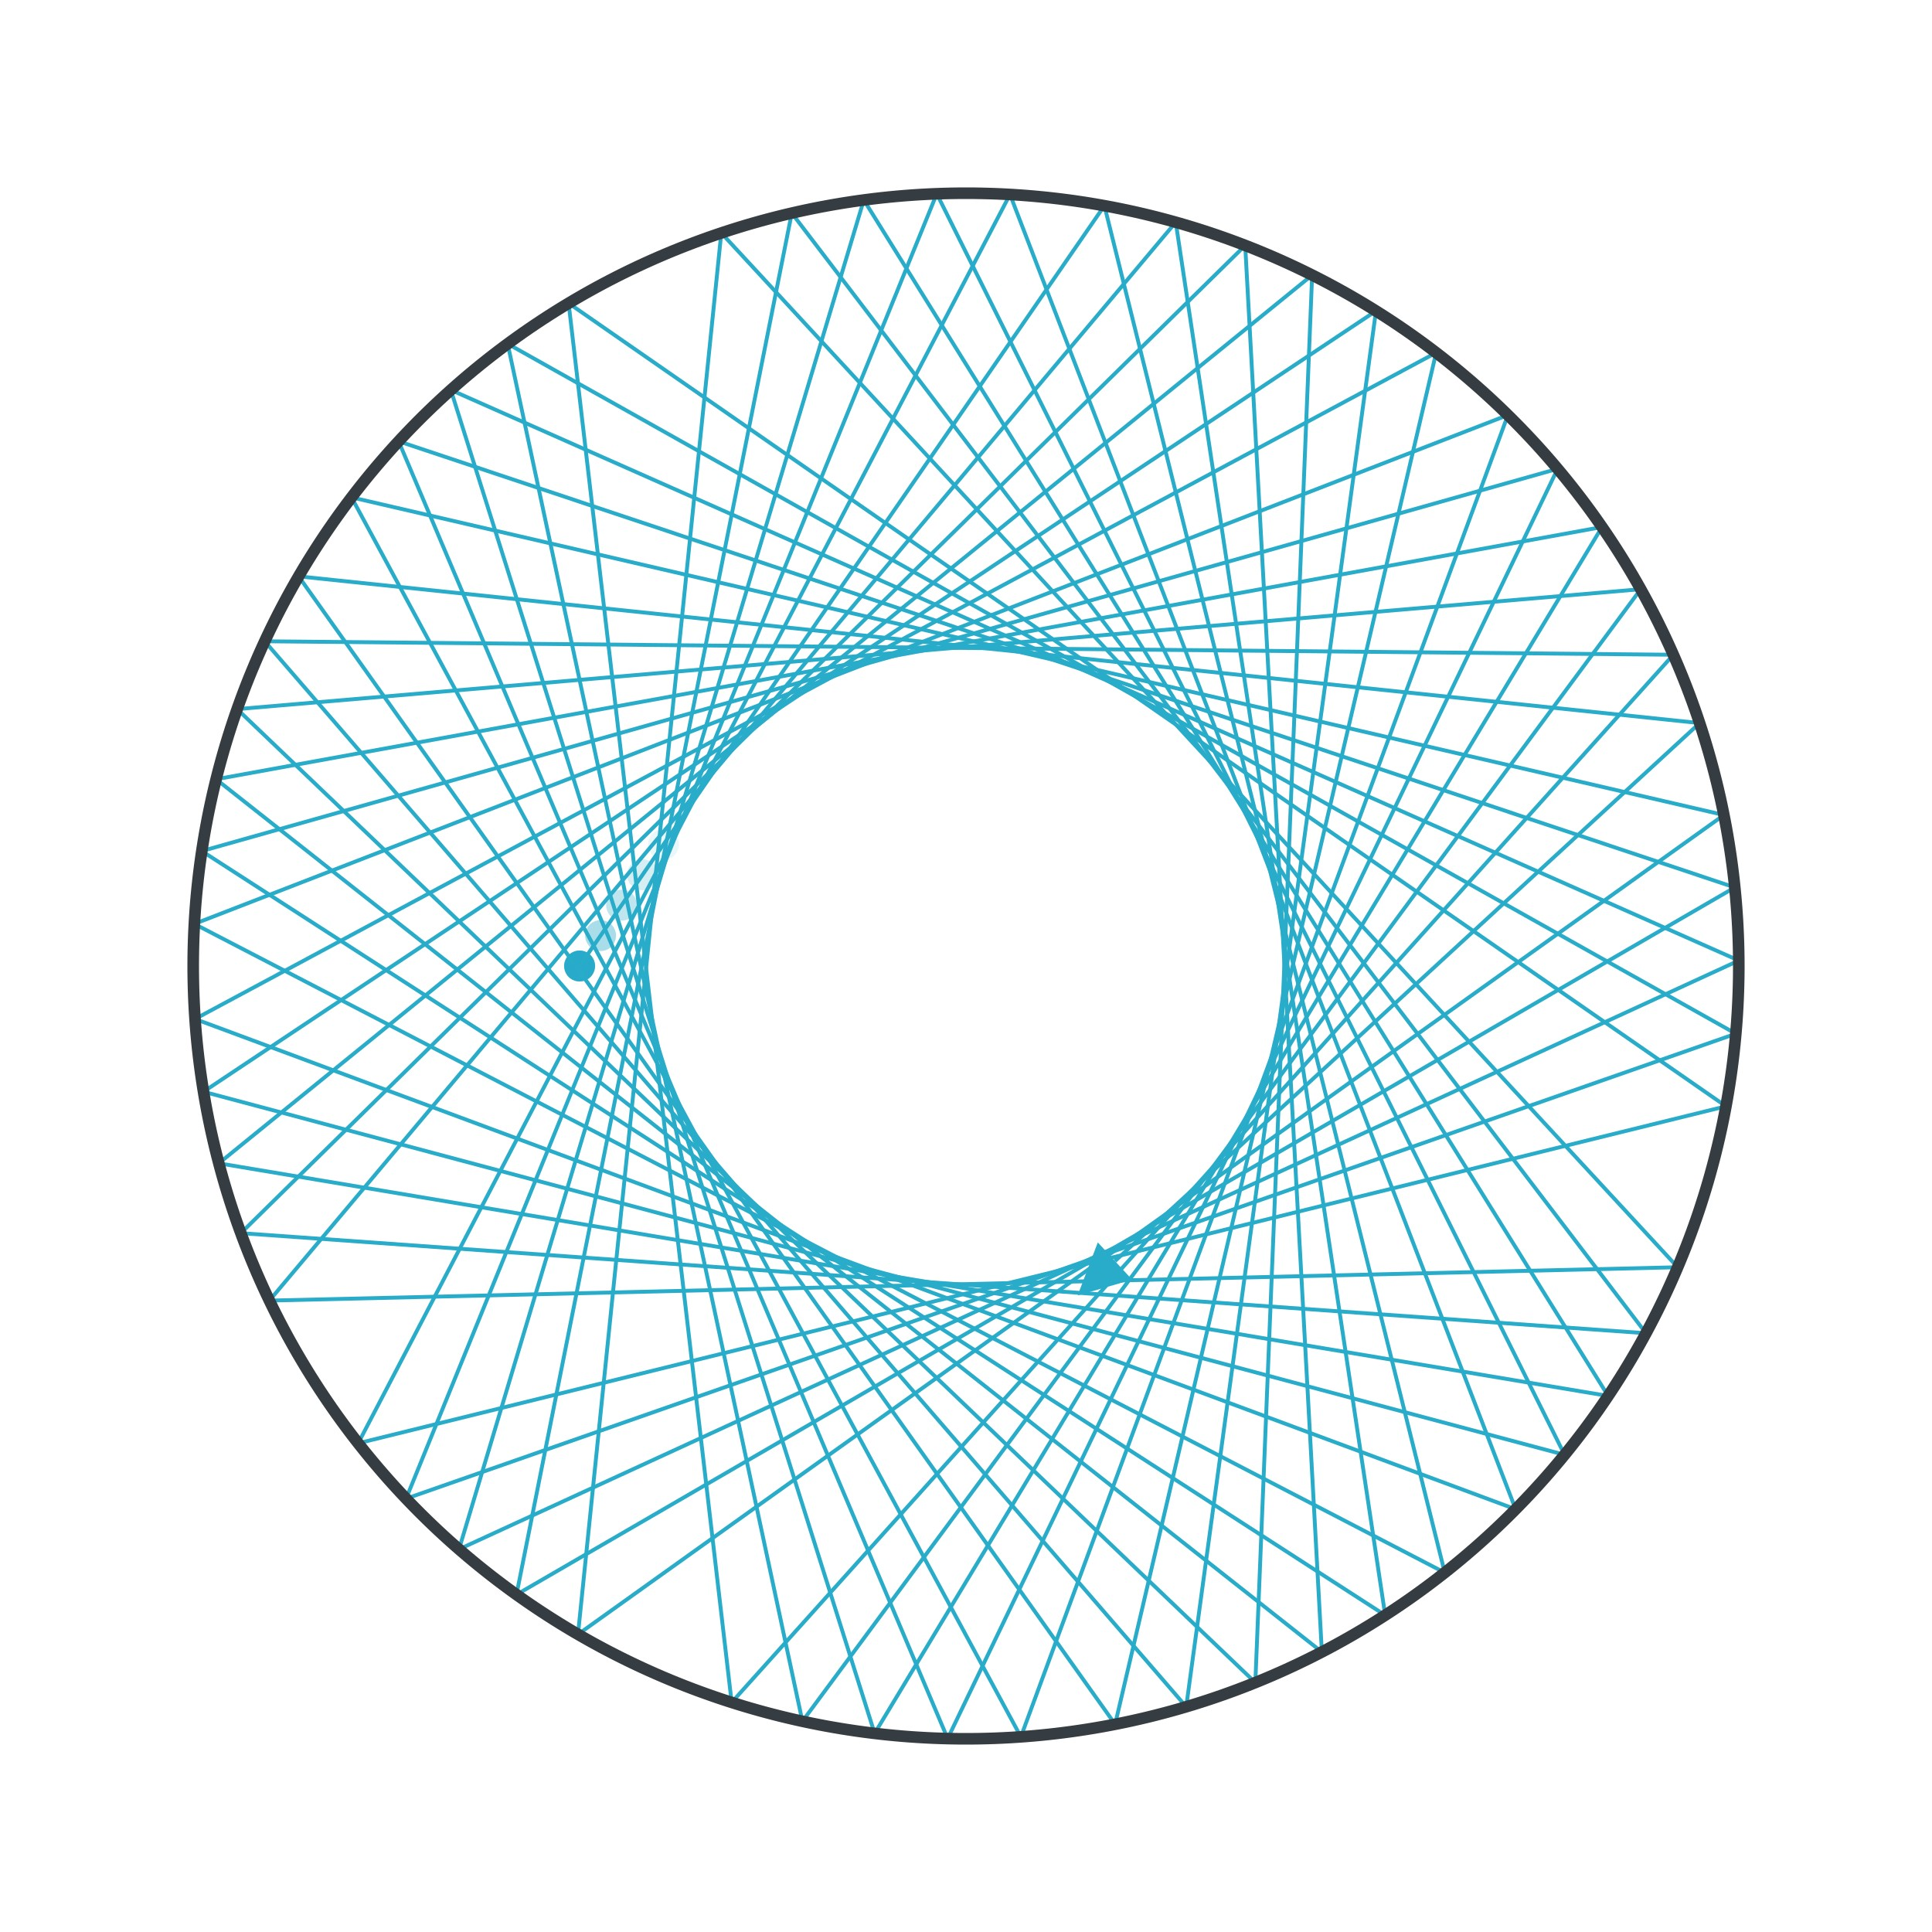
\includegraphics[scale=0.04,angle=0]{Circle_2.jpg}
    %\caption{Variabili $X_{n}$}
    \label{fig:circ1}
  \end{subfigure}
  %
  \begin{subfigure}[b]{0.3\textwidth}
  \centering
    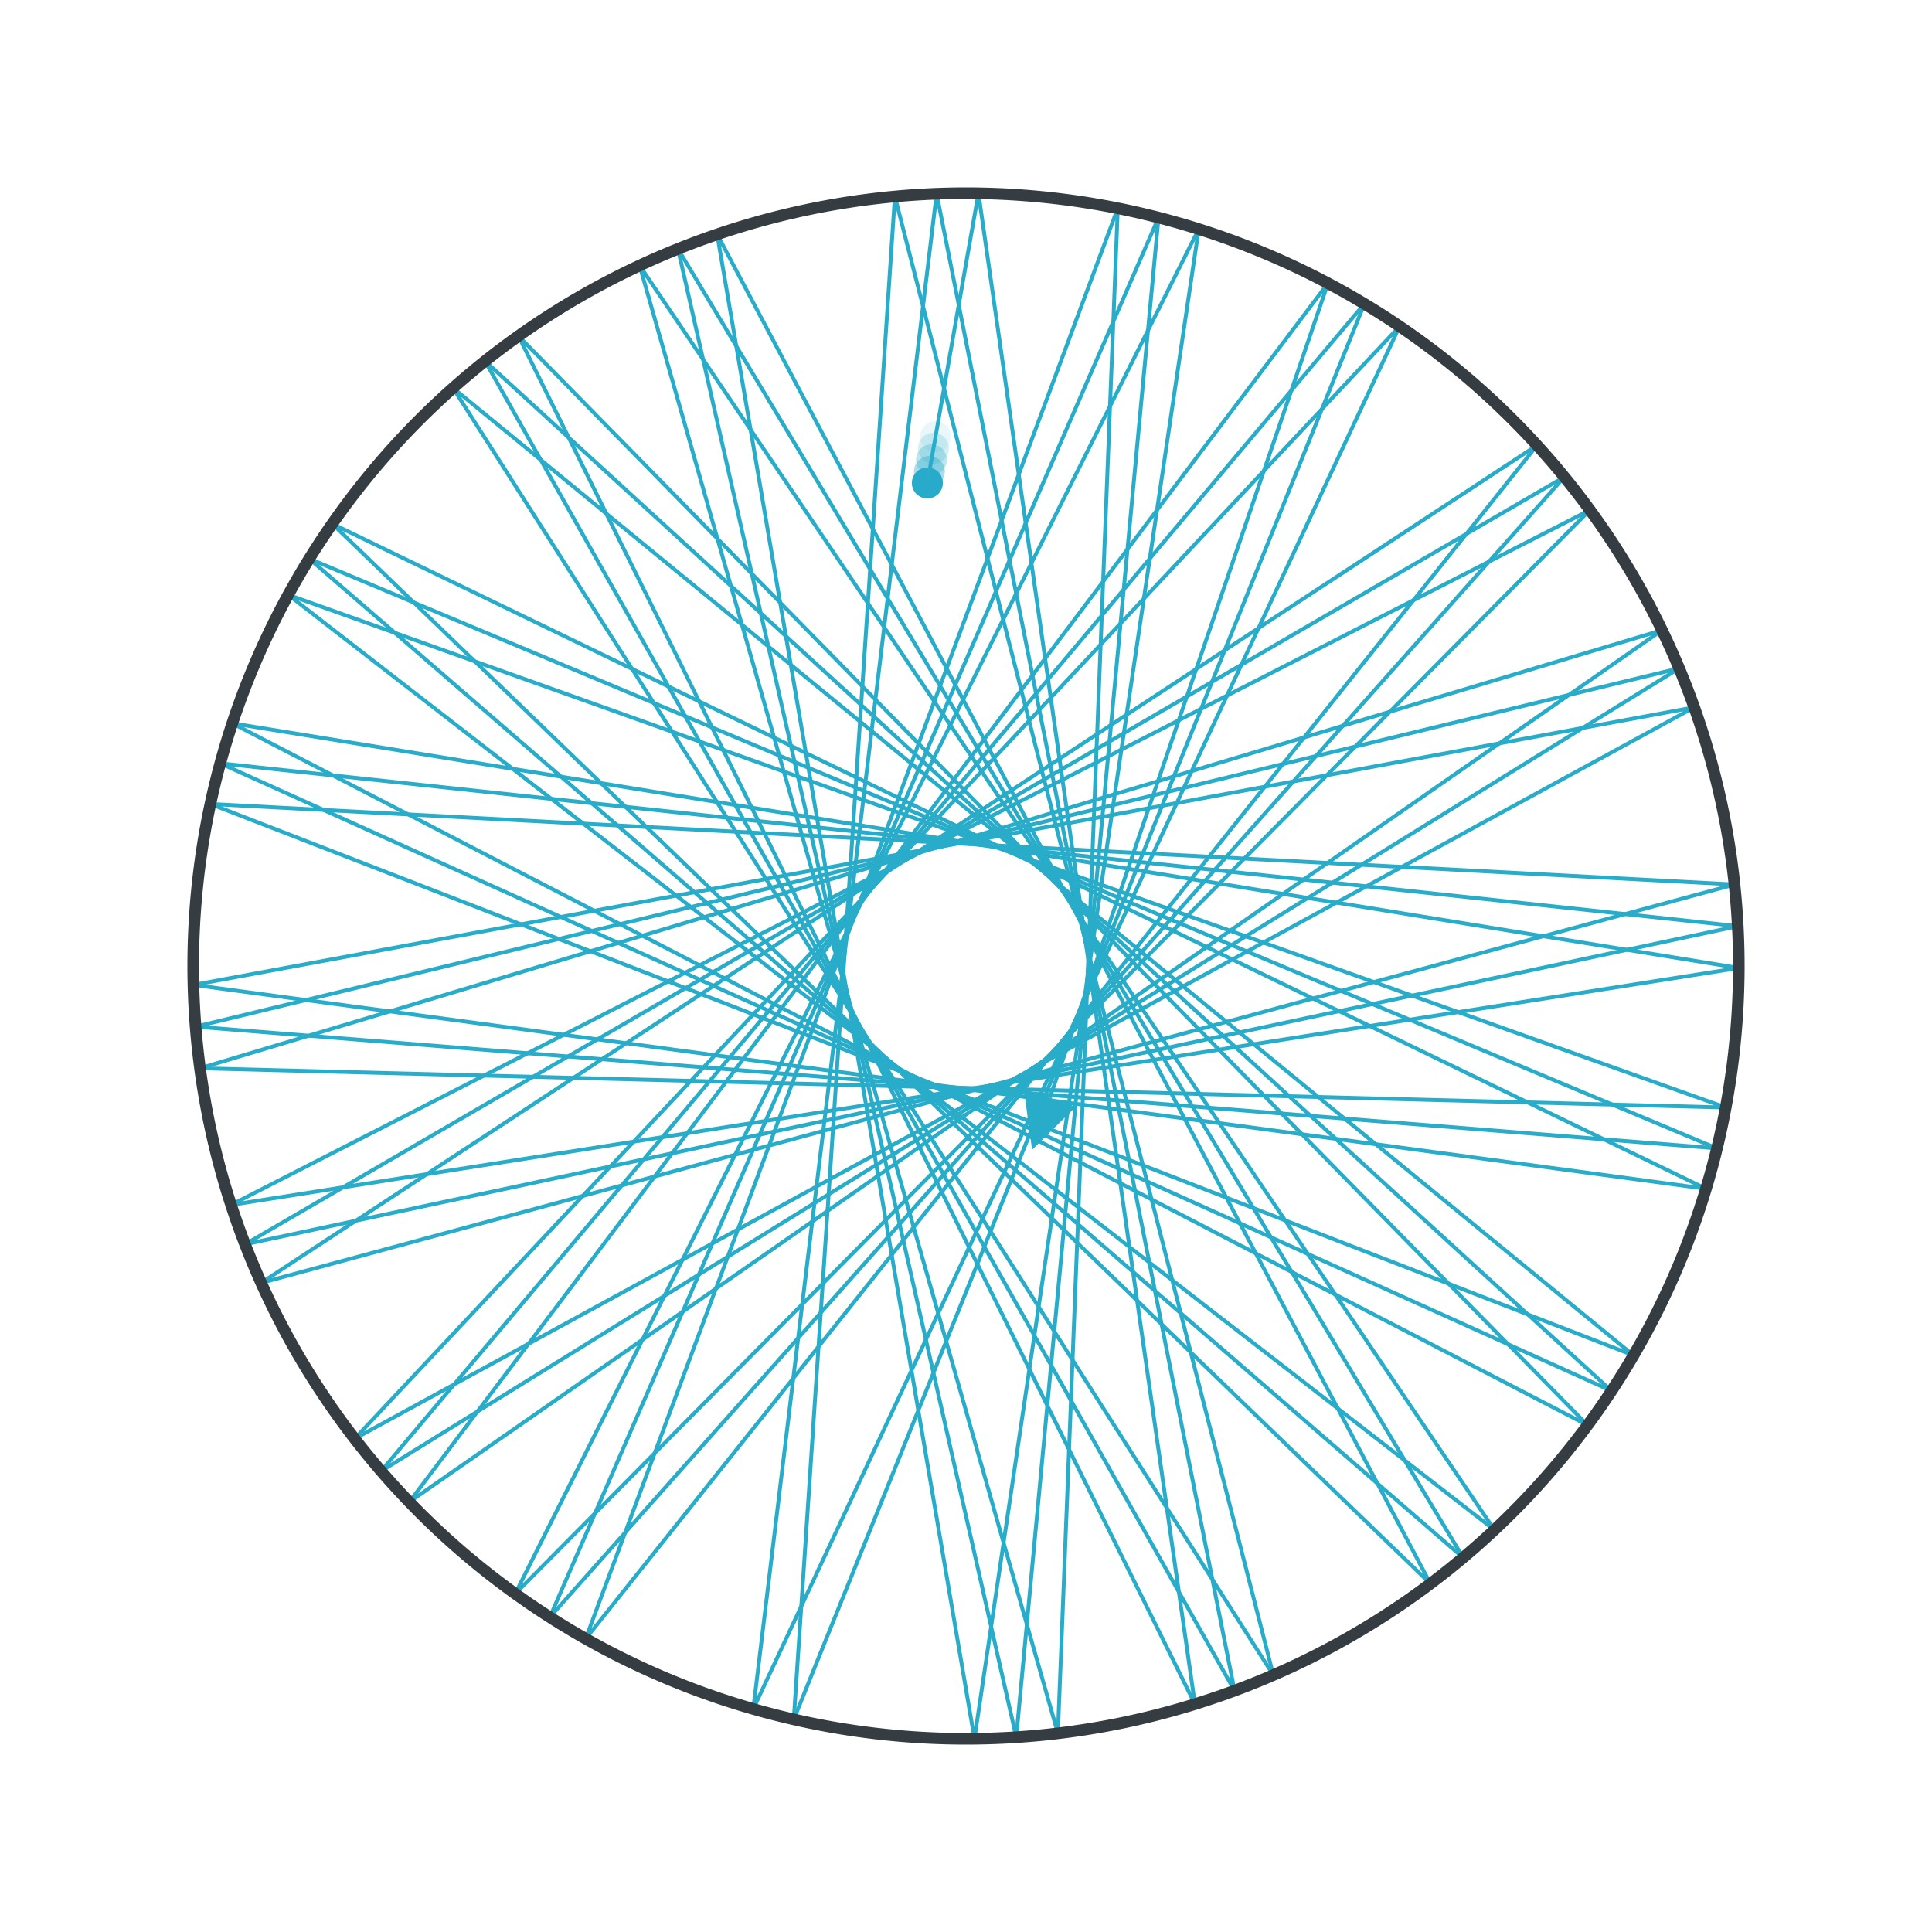
\includegraphics[scale=0.04,angle=0]{Circle_3.jpg}
    %\caption{Variabili $X_{n}$}
    \label{fig:circ2}
  \end{subfigure}
  \begin{subfigure}[b]{0.3\textwidth}
  \centering
    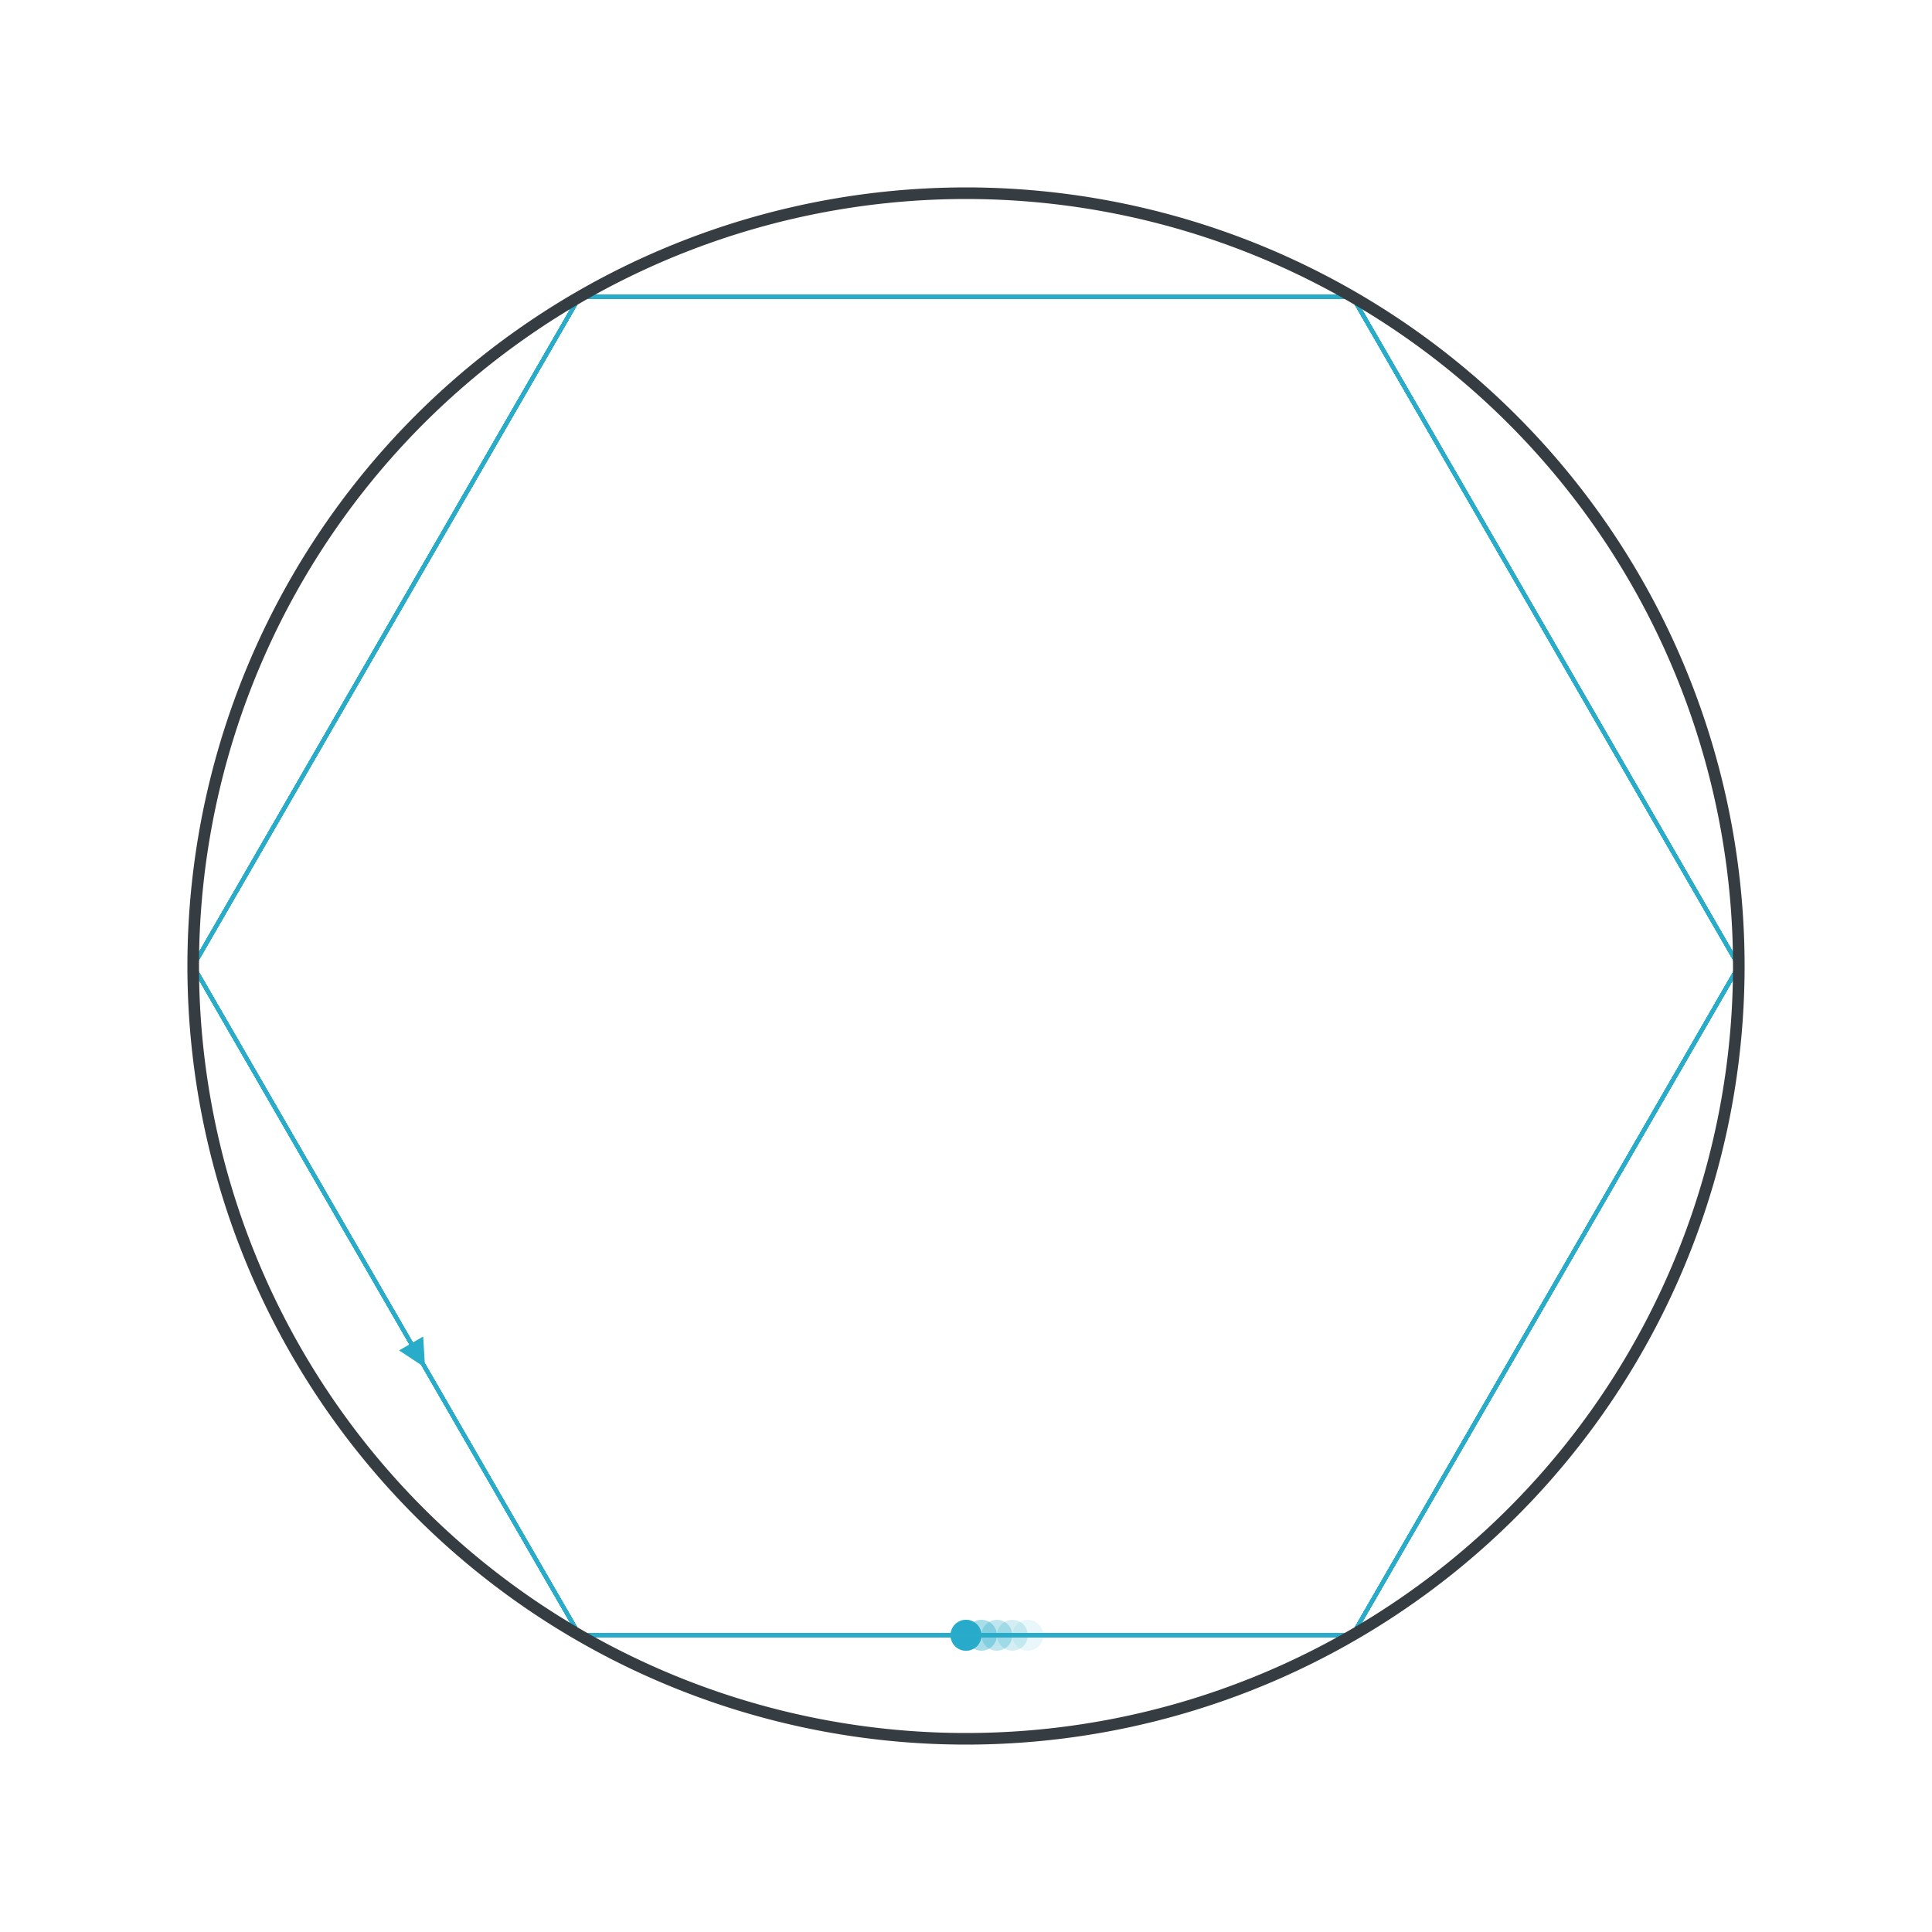
\includegraphics[scale=0.04,angle=0]{Circle_4.jpg}
    %\caption{Variabili $X_{n}$}
    \label{fig:circ3}
  \end{subfigure}
  \noindent\\
  \begin{subfigure}[b]{0.4\textwidth}
  \centering
    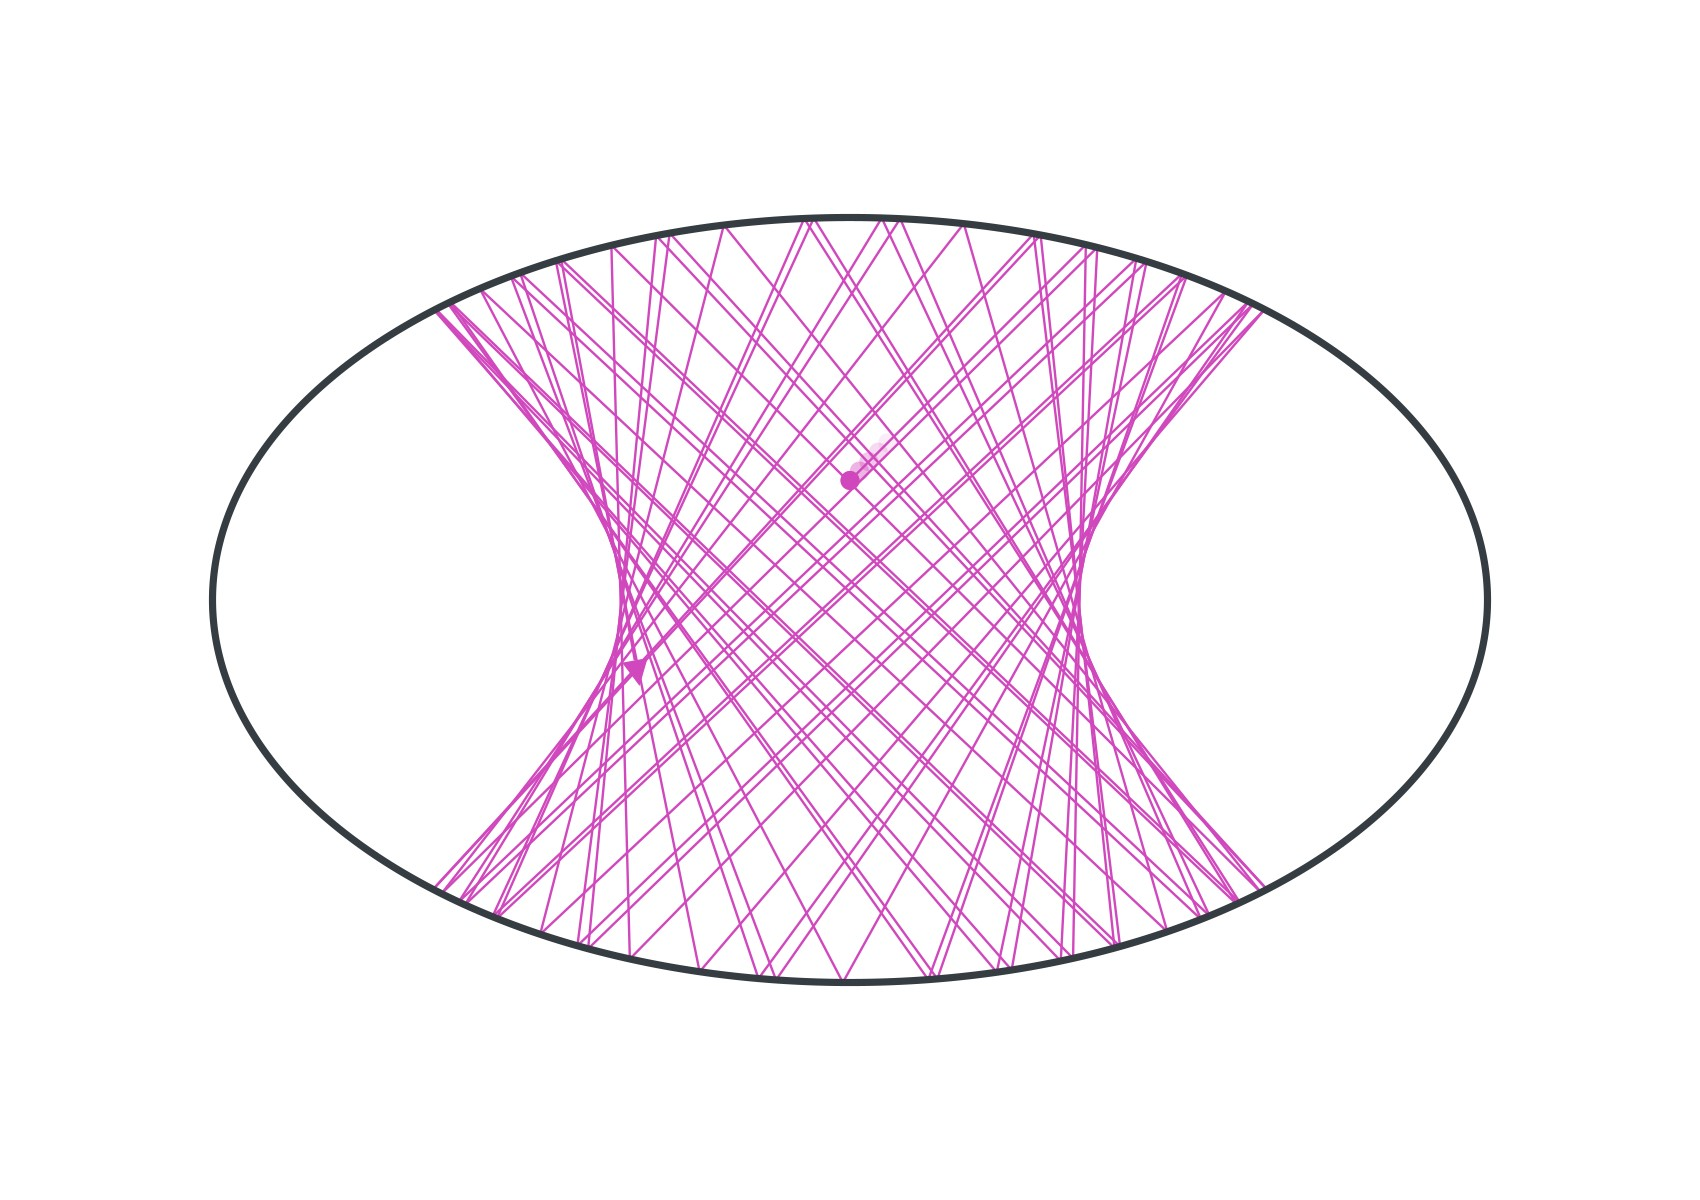
\includegraphics[scale=0.08,angle=0]{Ellipse1.jpg}
    %\caption{Variabili $X_{n}$}
    \label{fig:ellip1}
  \end{subfigure}
  \begin{subfigure}[b]{0.4\textwidth}
  \centering
    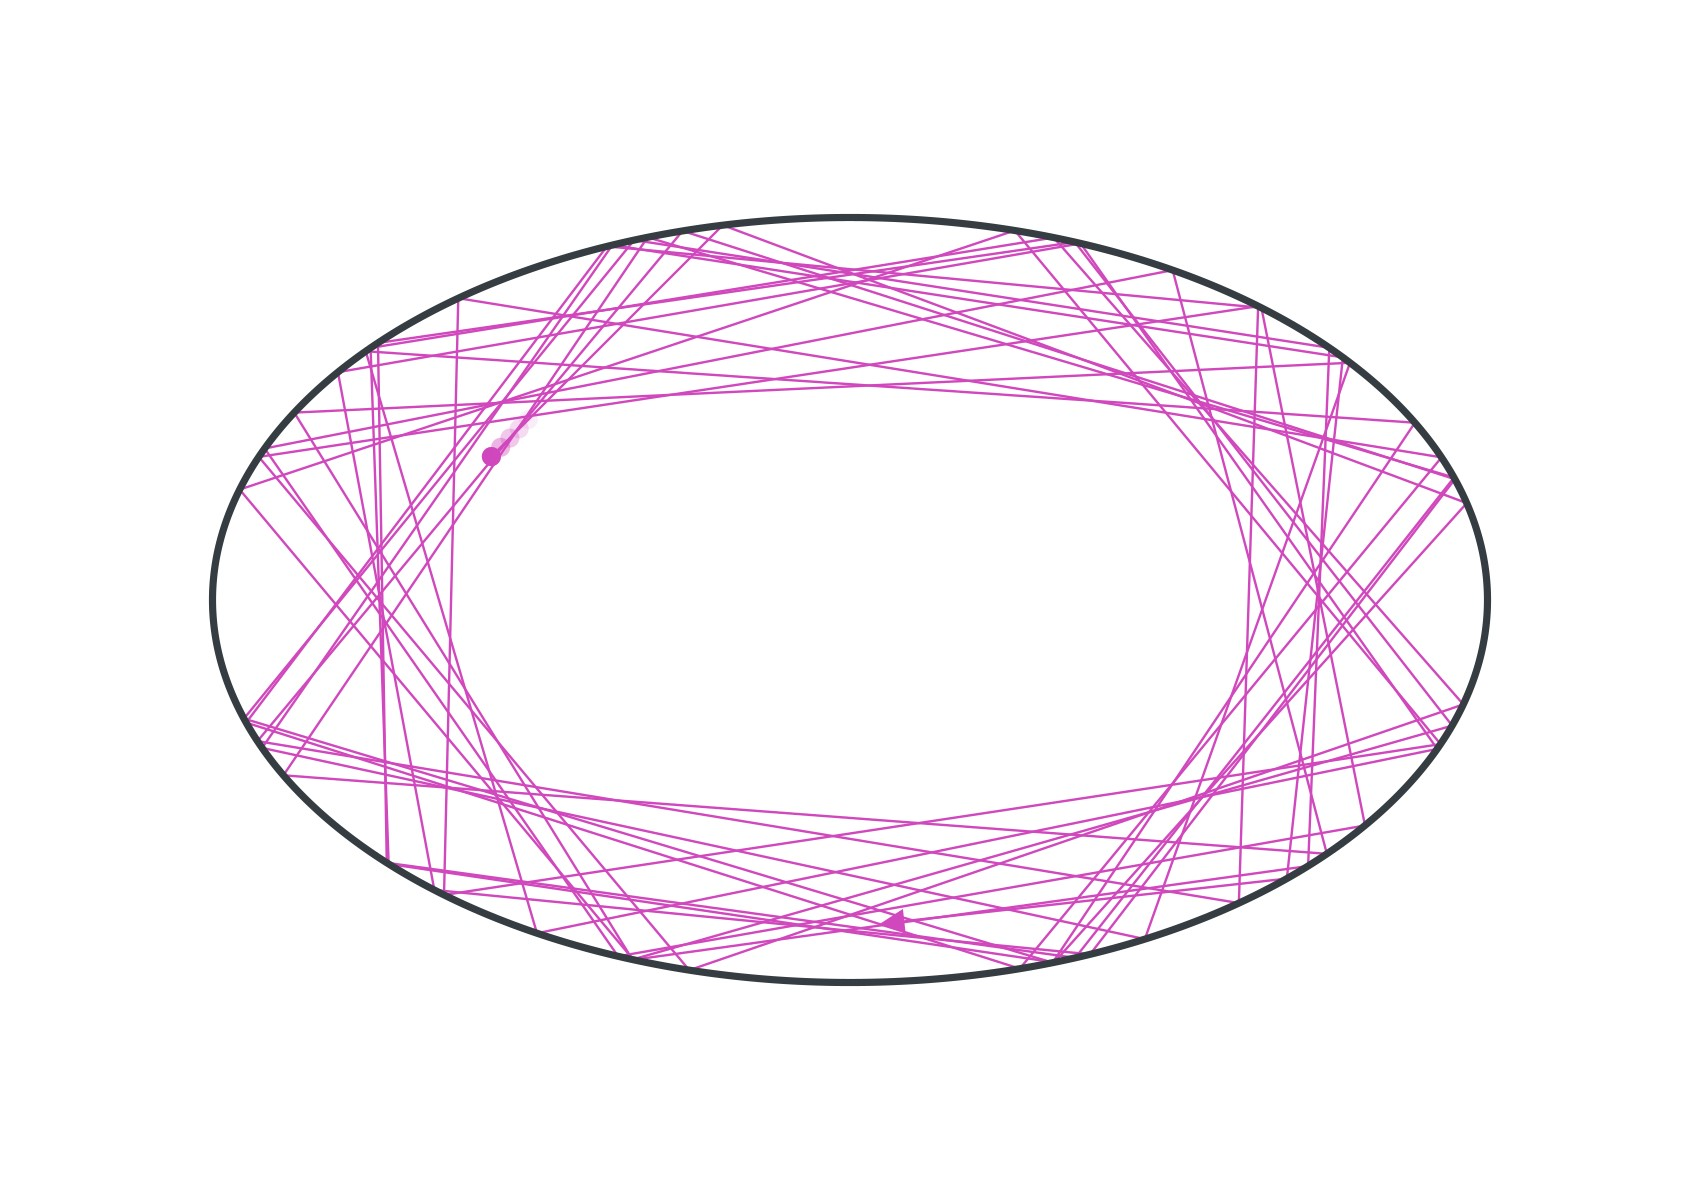
\includegraphics[scale=0.08,angle=0]{Ellipse2.jpg}
    %\caption{Variabili $X_{n}$}
    \label{fig:ellip2}
  \end{subfigure}
  \noindent\\
  \decoRule
  \caption{Billiard trajectories on a circle and an ellipse. The underlying system is conservative, hence the motion is not \virg{everywhere distributed}.}
  \label{fig:ell_circ_billiards}
\end{figure}


The followings are examples of ergodic billiards.

\begin{nese}[Bunimovich stadium]
\label{ese:bunimovich_stadium}
This billard is by far the most famous one and the most studied in details. Albeit it may seem contrived, this billiard is full of remarkable properties and so it is considered the fundamental prototype for a chaotic billiard. The domain $\Omega$ is made up by one rectangle and two half-circles on two sides. This billiard is ergodic and mixing. Moreover, it is also \virg{chaotic} in the sense that \virg{near trajectories} have drammatically different time-evolution (see figure \ref{fig:bunimovich_orbits})\\
We will denote by $\BS_{l}$ the Bunimovich stadium defined by the rectangle $\left[
-l\frac{\pi}{2},l\frac{\pi}{2}
\right]\times
\left[
-\frac{\pi}{2},\frac{\pi}{2}
\right]$ and the two semicircle of radius $\pi/2$.
\end{nese}


\begin{figure}[H]
\centering
  \begin{subfigure}[b]{0.7\textwidth}
  \centering
    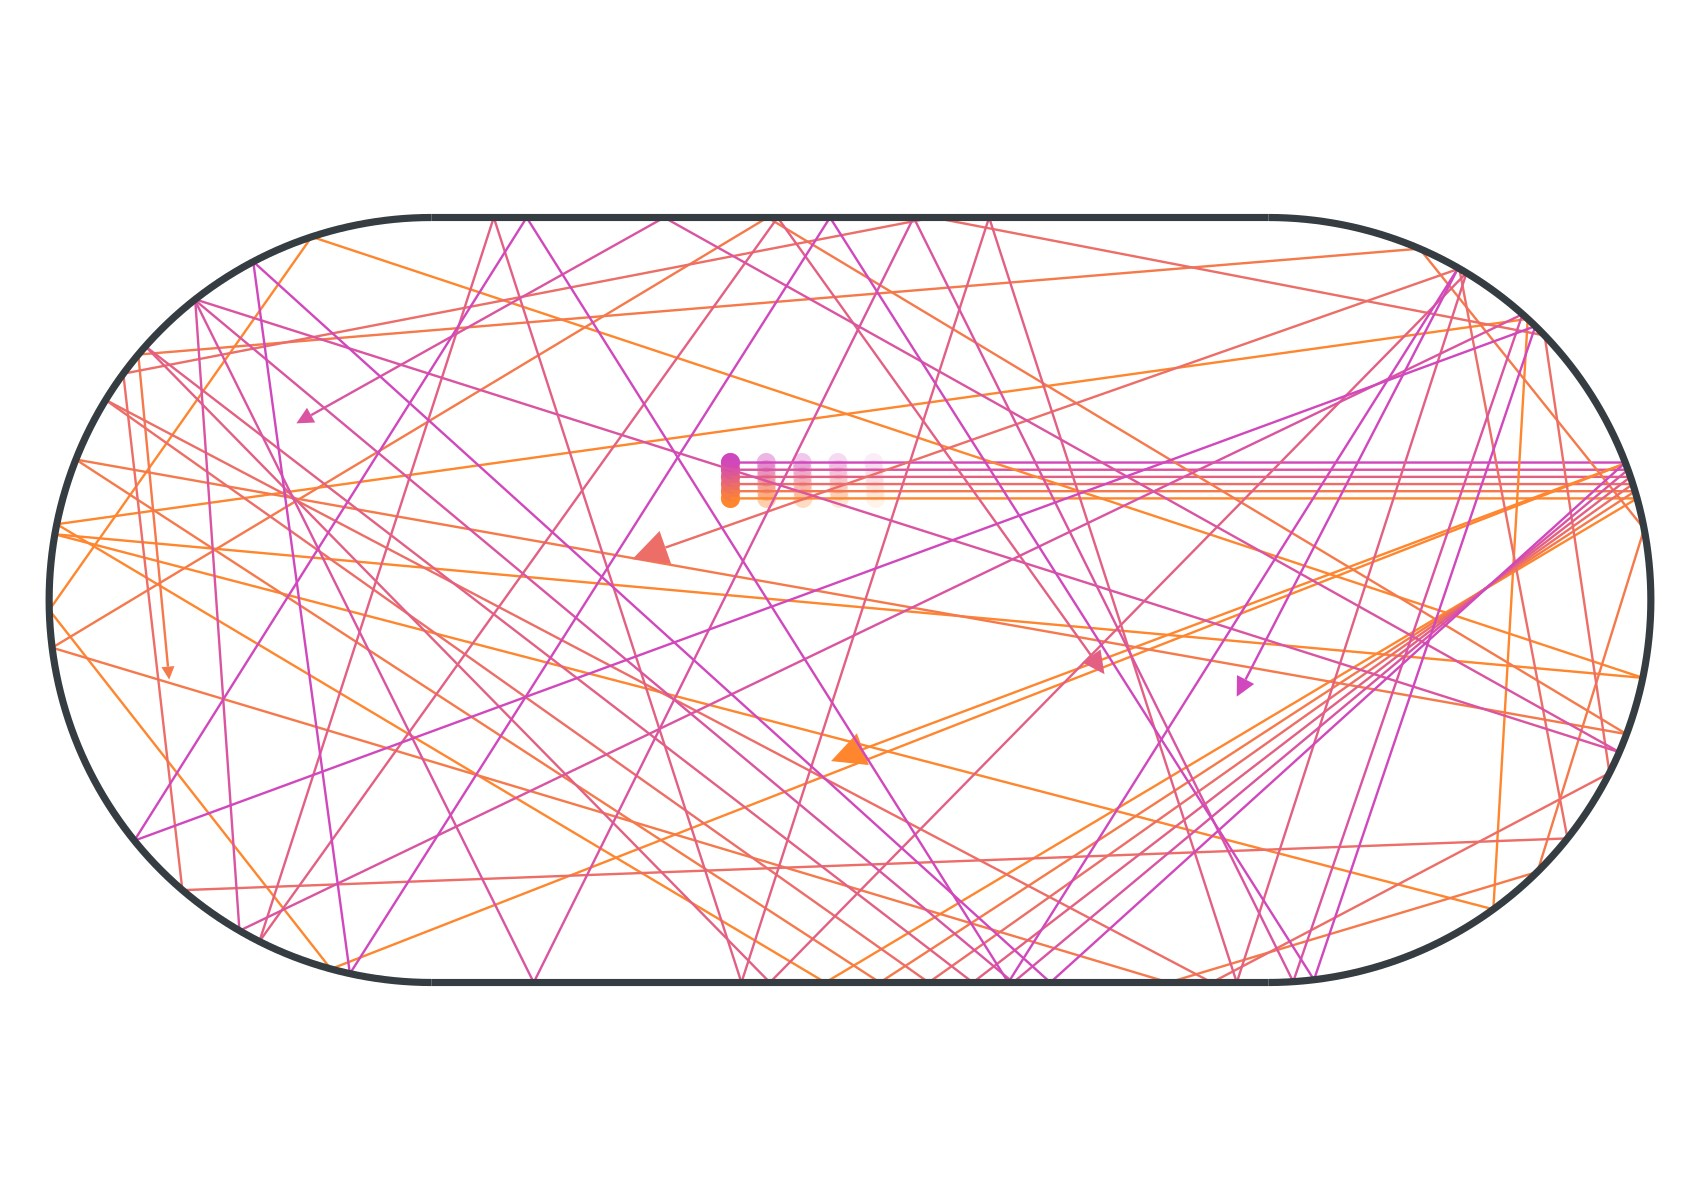
\includegraphics[scale=0.11,angle=0]{Stadium_diverg.jpg}
    %\caption{Variabili $X_{n}$}
    \label{fig:bun1}
  \end{subfigure}
  %
  \noindent\\
  \begin{subfigure}[b]{0.3\textwidth}
  \centering
    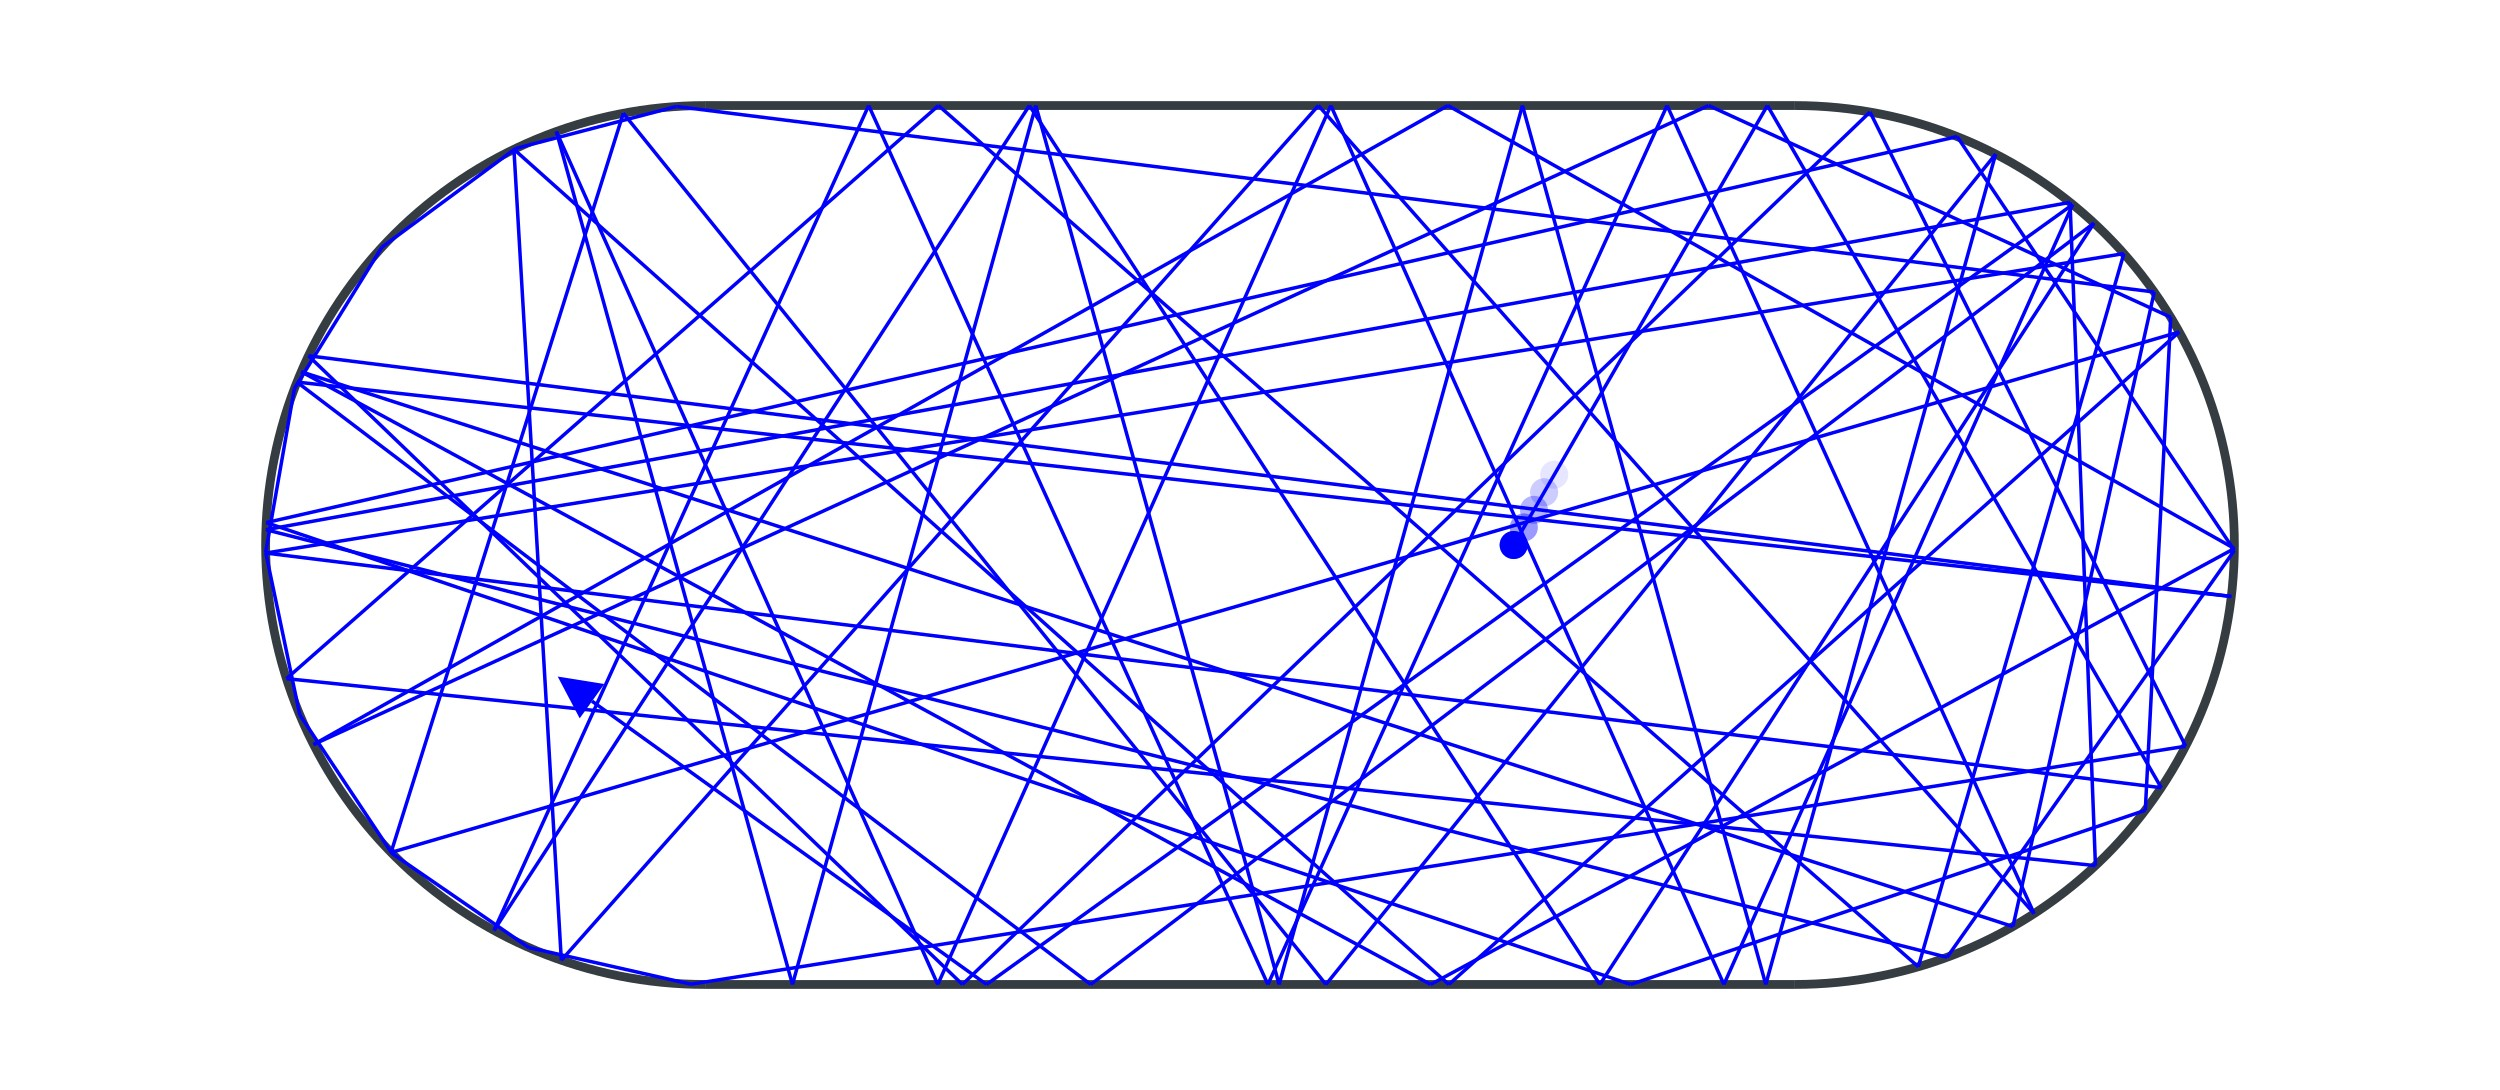
\includegraphics[scale=0.05,angle=0]{Stad_2.jpg}
    %\caption{Variabili $X_{n}$}
    \label{fig:bun2}
  \end{subfigure}
  \begin{subfigure}[b]{0.3\textwidth}
  \centering
    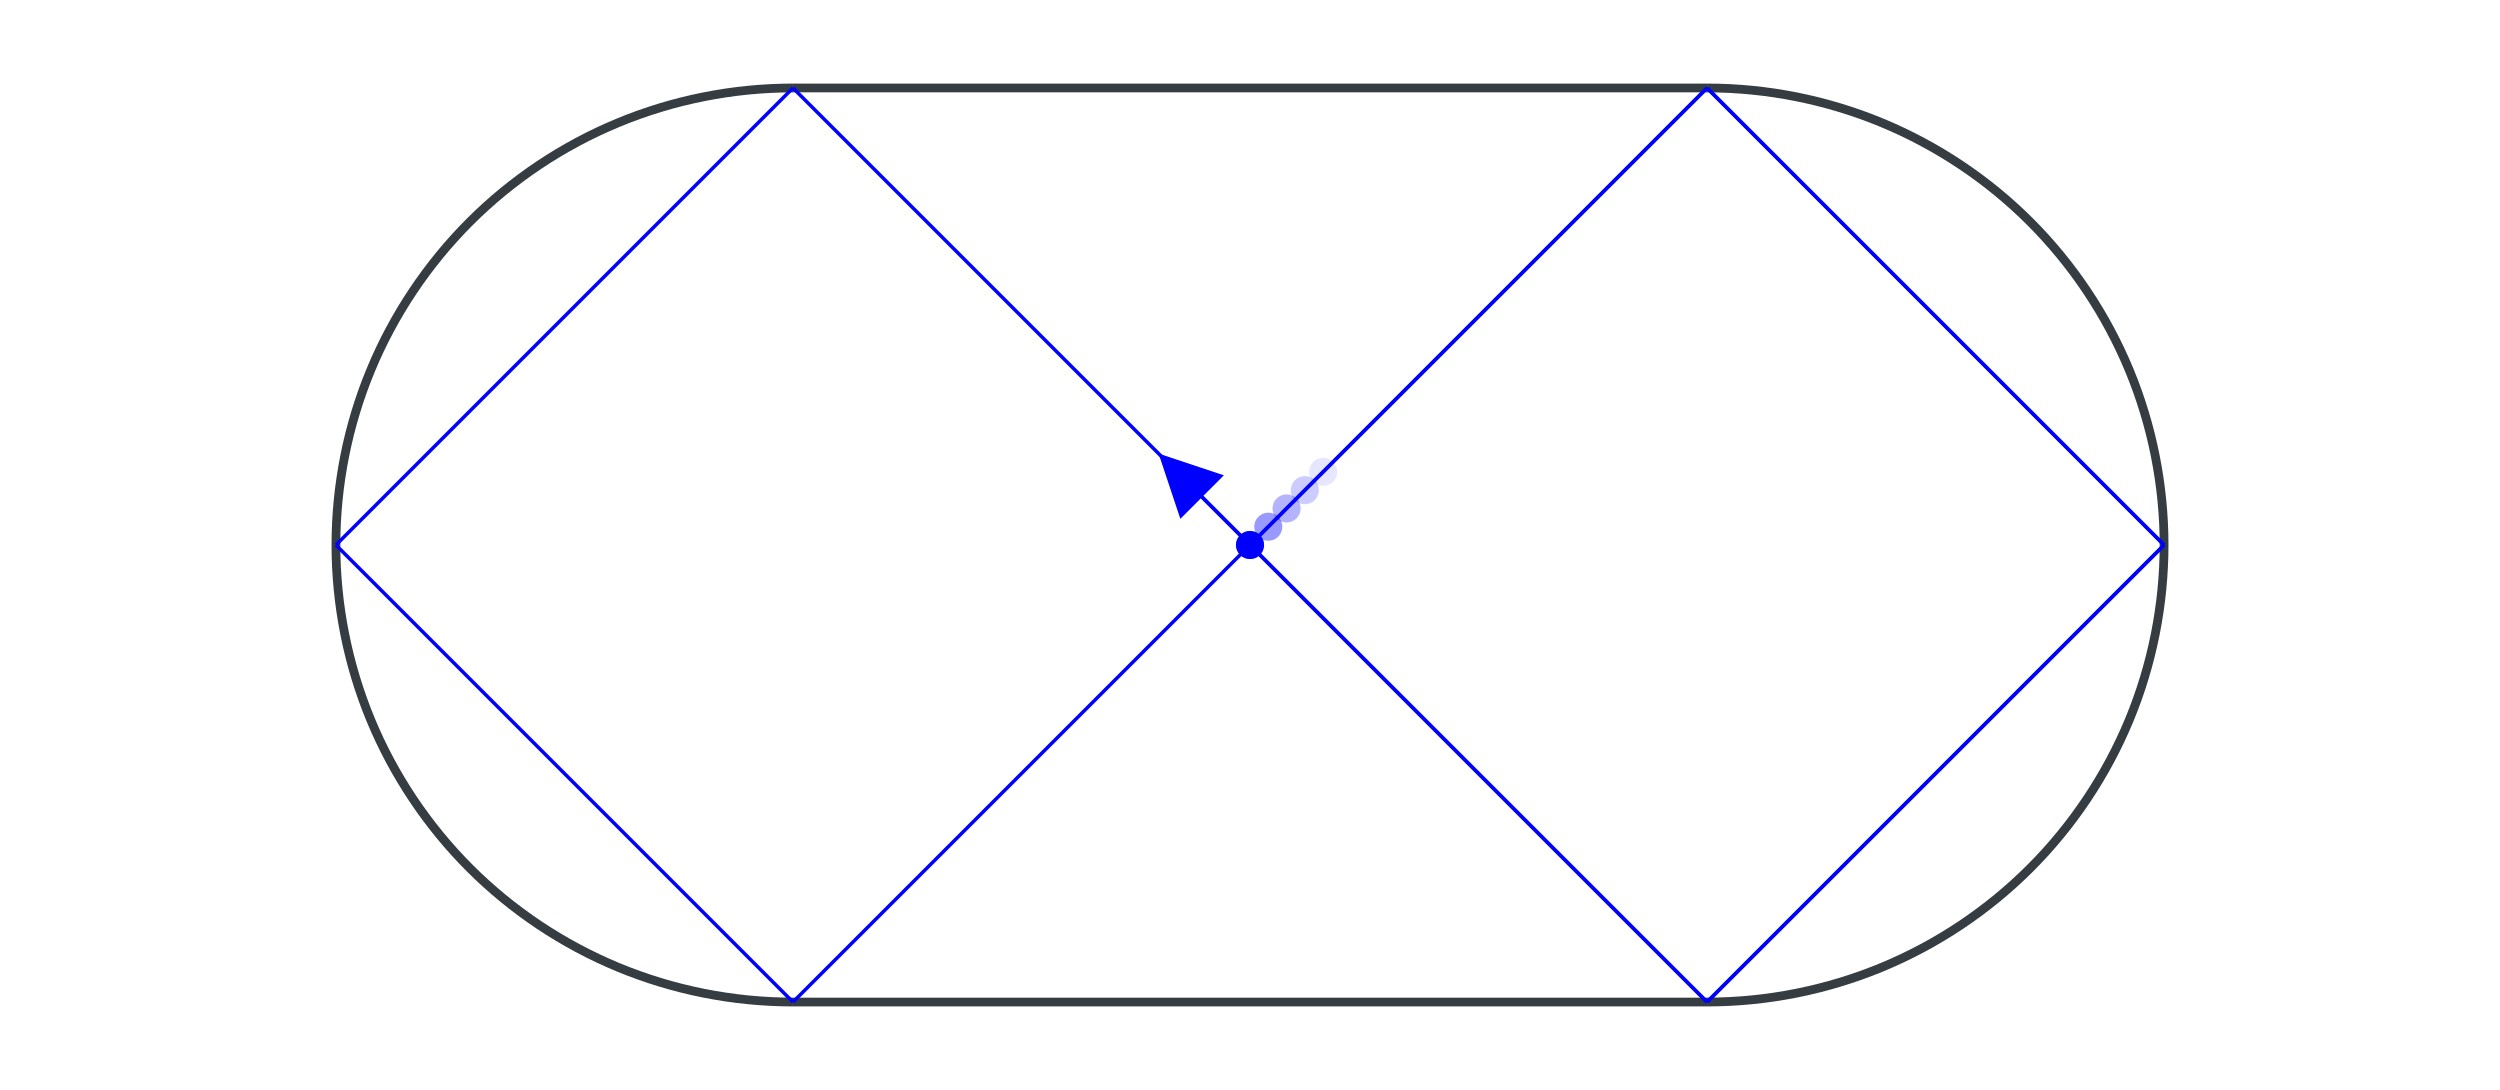
\includegraphics[scale=0.05,angle=0]{Stad_3.jpg}
    %\caption{Variabili $X_{n}$}
    \label{fig:bun3}
  \end{subfigure}
  \noindent\\
  \decoRule
  \caption{Billiard trajectories on the Bunimovich stadium.}
  \label{fig:bunimovich_orbits}
\end{figure}


\begin{nese}[Barnett's billiard]
This billiard is made up by two circle arcs and two perpendicular segment. The circle arcs must intersect creating an acute angle. Peter Sarnak called this billiard \virg{Barnett's billiard}, thanks to the latter's numerical studies on this billiard. We will denote the generic Barnett's billiard with $\BarS$. It is mixing and, moreover, Sinai proved that near orbits diverge exponentially.
\end{nese}


\begin{figure}[H]
\centering
  \begin{subfigure}[b]{0.7\textwidth}
  \centering
    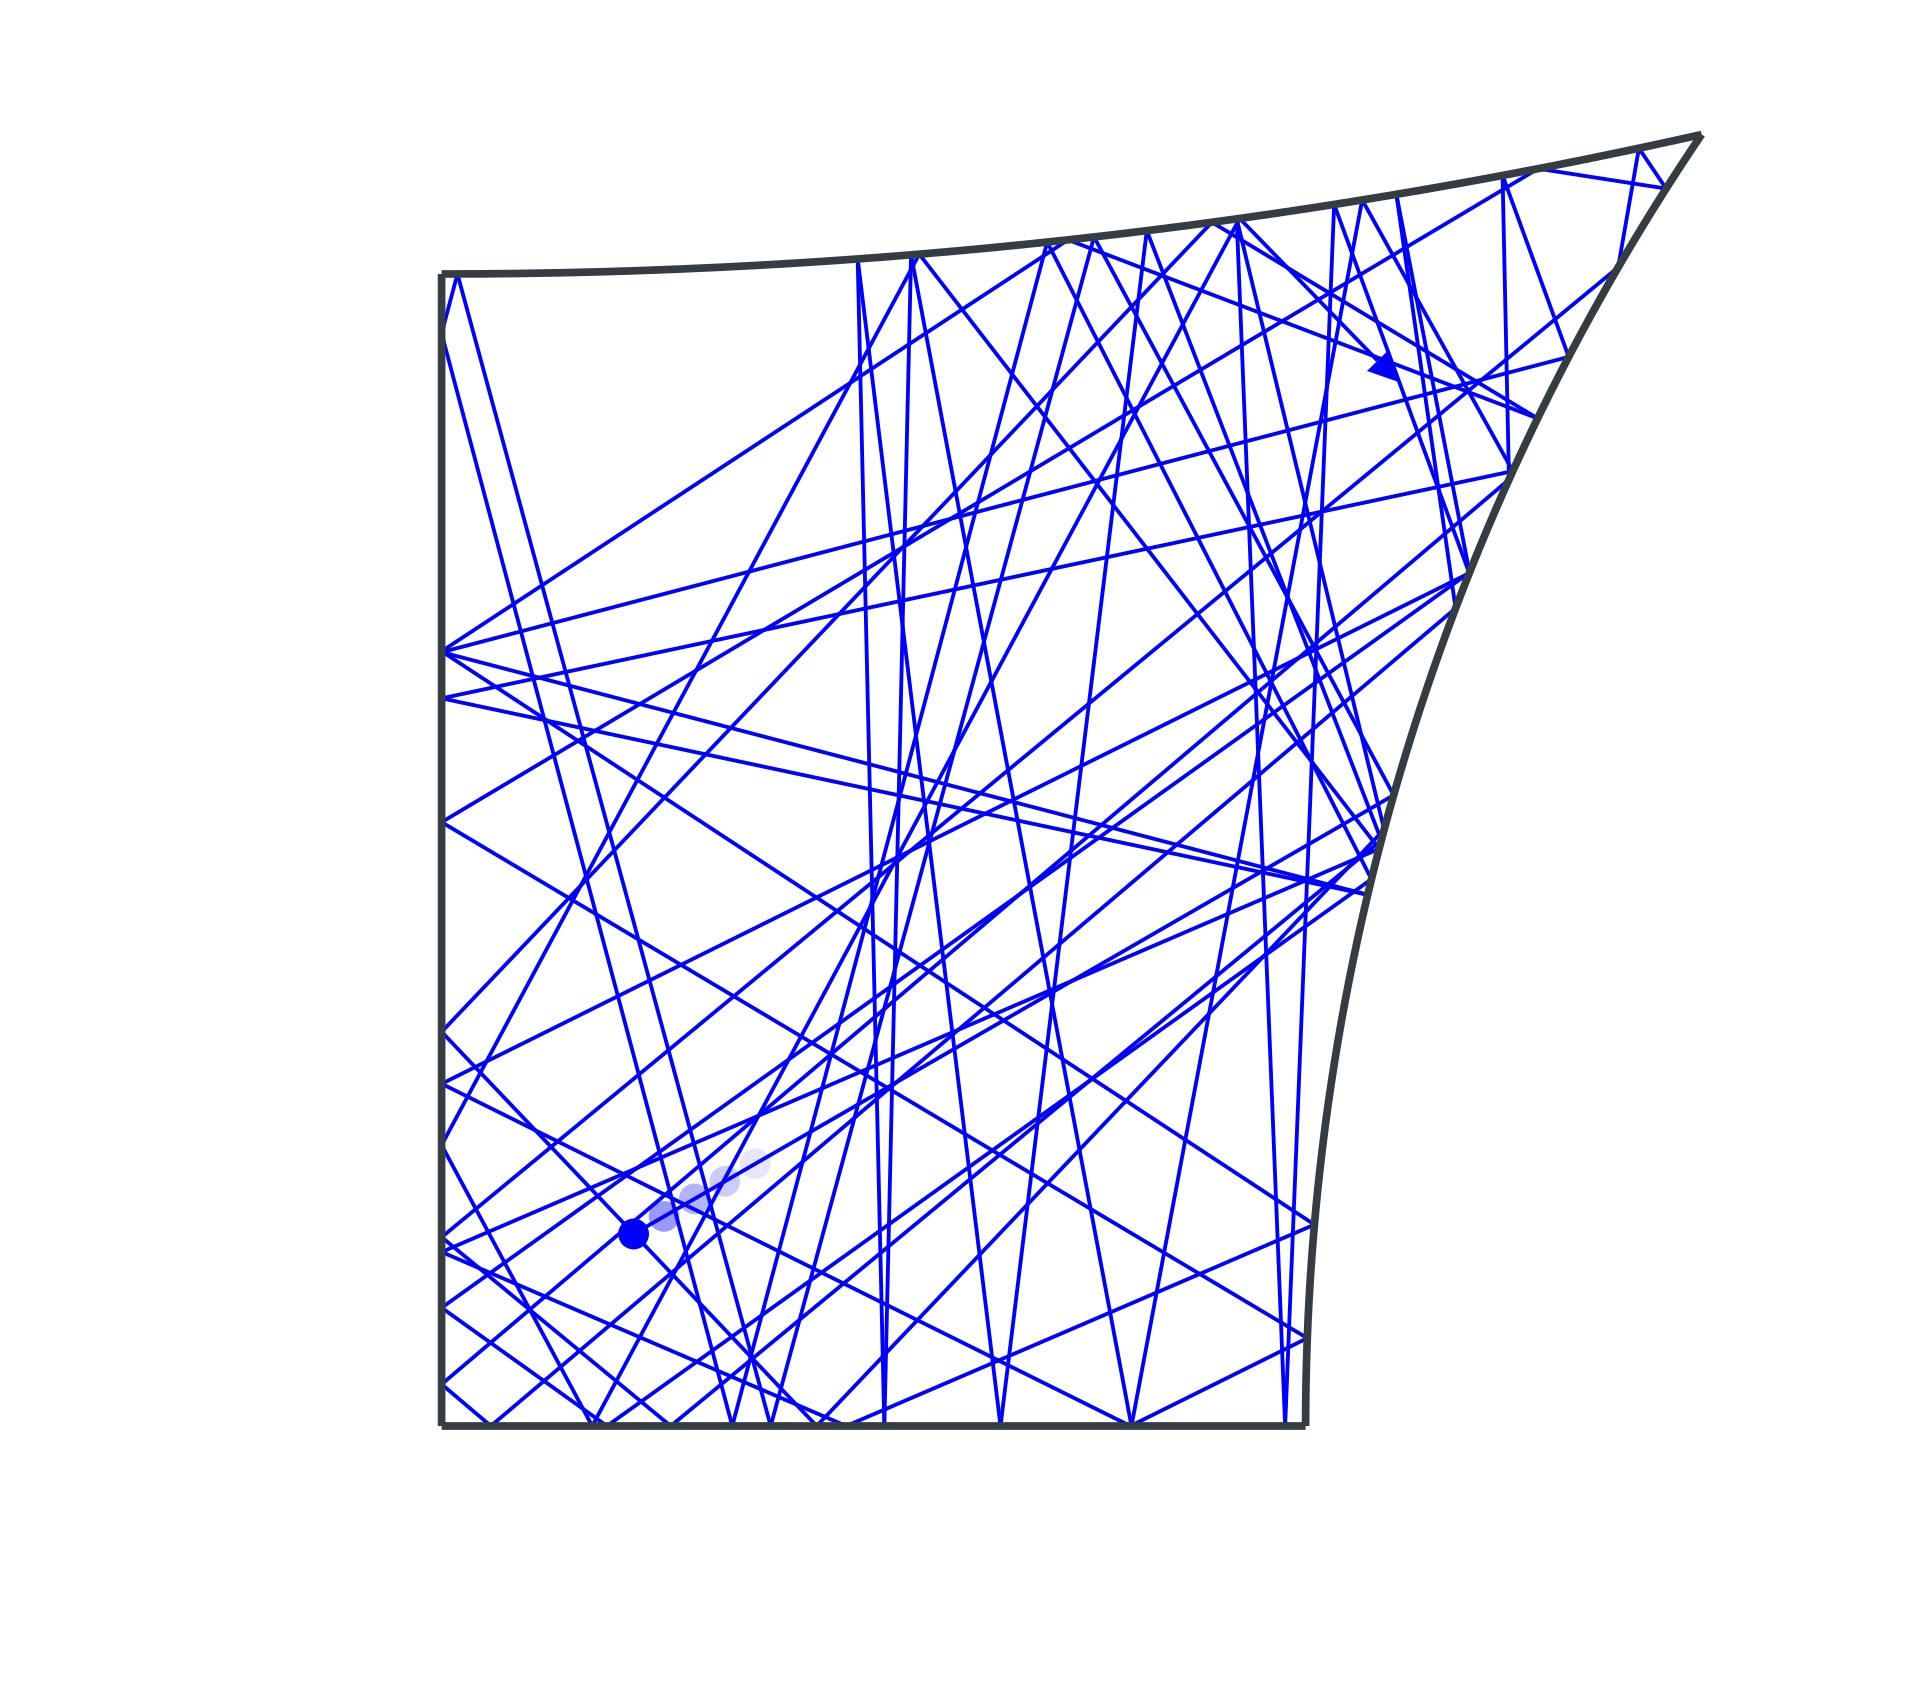
\includegraphics[scale=0.08,angle=0]{Barnett2.jpg}
    %\caption{Variabili $X_{n}$}
    \label{fig:barn1}
  \end{subfigure}
  %
  \noindent\\
  \decoRule
  \caption{Barnett's billiard.}
  \label{fig:barn_orbits}
\end{figure}

\begin{nese}[Cassini's billiard and cardioid billiard]
Other interesting billiards, which numerically share lots of properties of Bunimovich and Barnett billiards are the Cardioid billiard $\CS_{r}$, with domain defined by the cardioid of (polar) equation
\[
\rho(\theta)=r(1-\cos\theta)
\]
and the Cassini's oval billiard $\COS_{a,b}$ defined by the equation
\[
(x^{2}+y^{2})^{2}-2\cdot a^{2}(x^{2}-y^{2})+a^{4}=b^{4}, \quad a,b>0,\, b>a.
\]
In particular, for $b/a\geq\sqrt{2}$ is convex, otherwise for $1<b/a<\sqrt{2}$ it is peanut-shaped.
\end{nese}

\begin{figure}[H]
\centering
  %
  \begin{subfigure}[b]{0.5\textwidth}
  \centering
    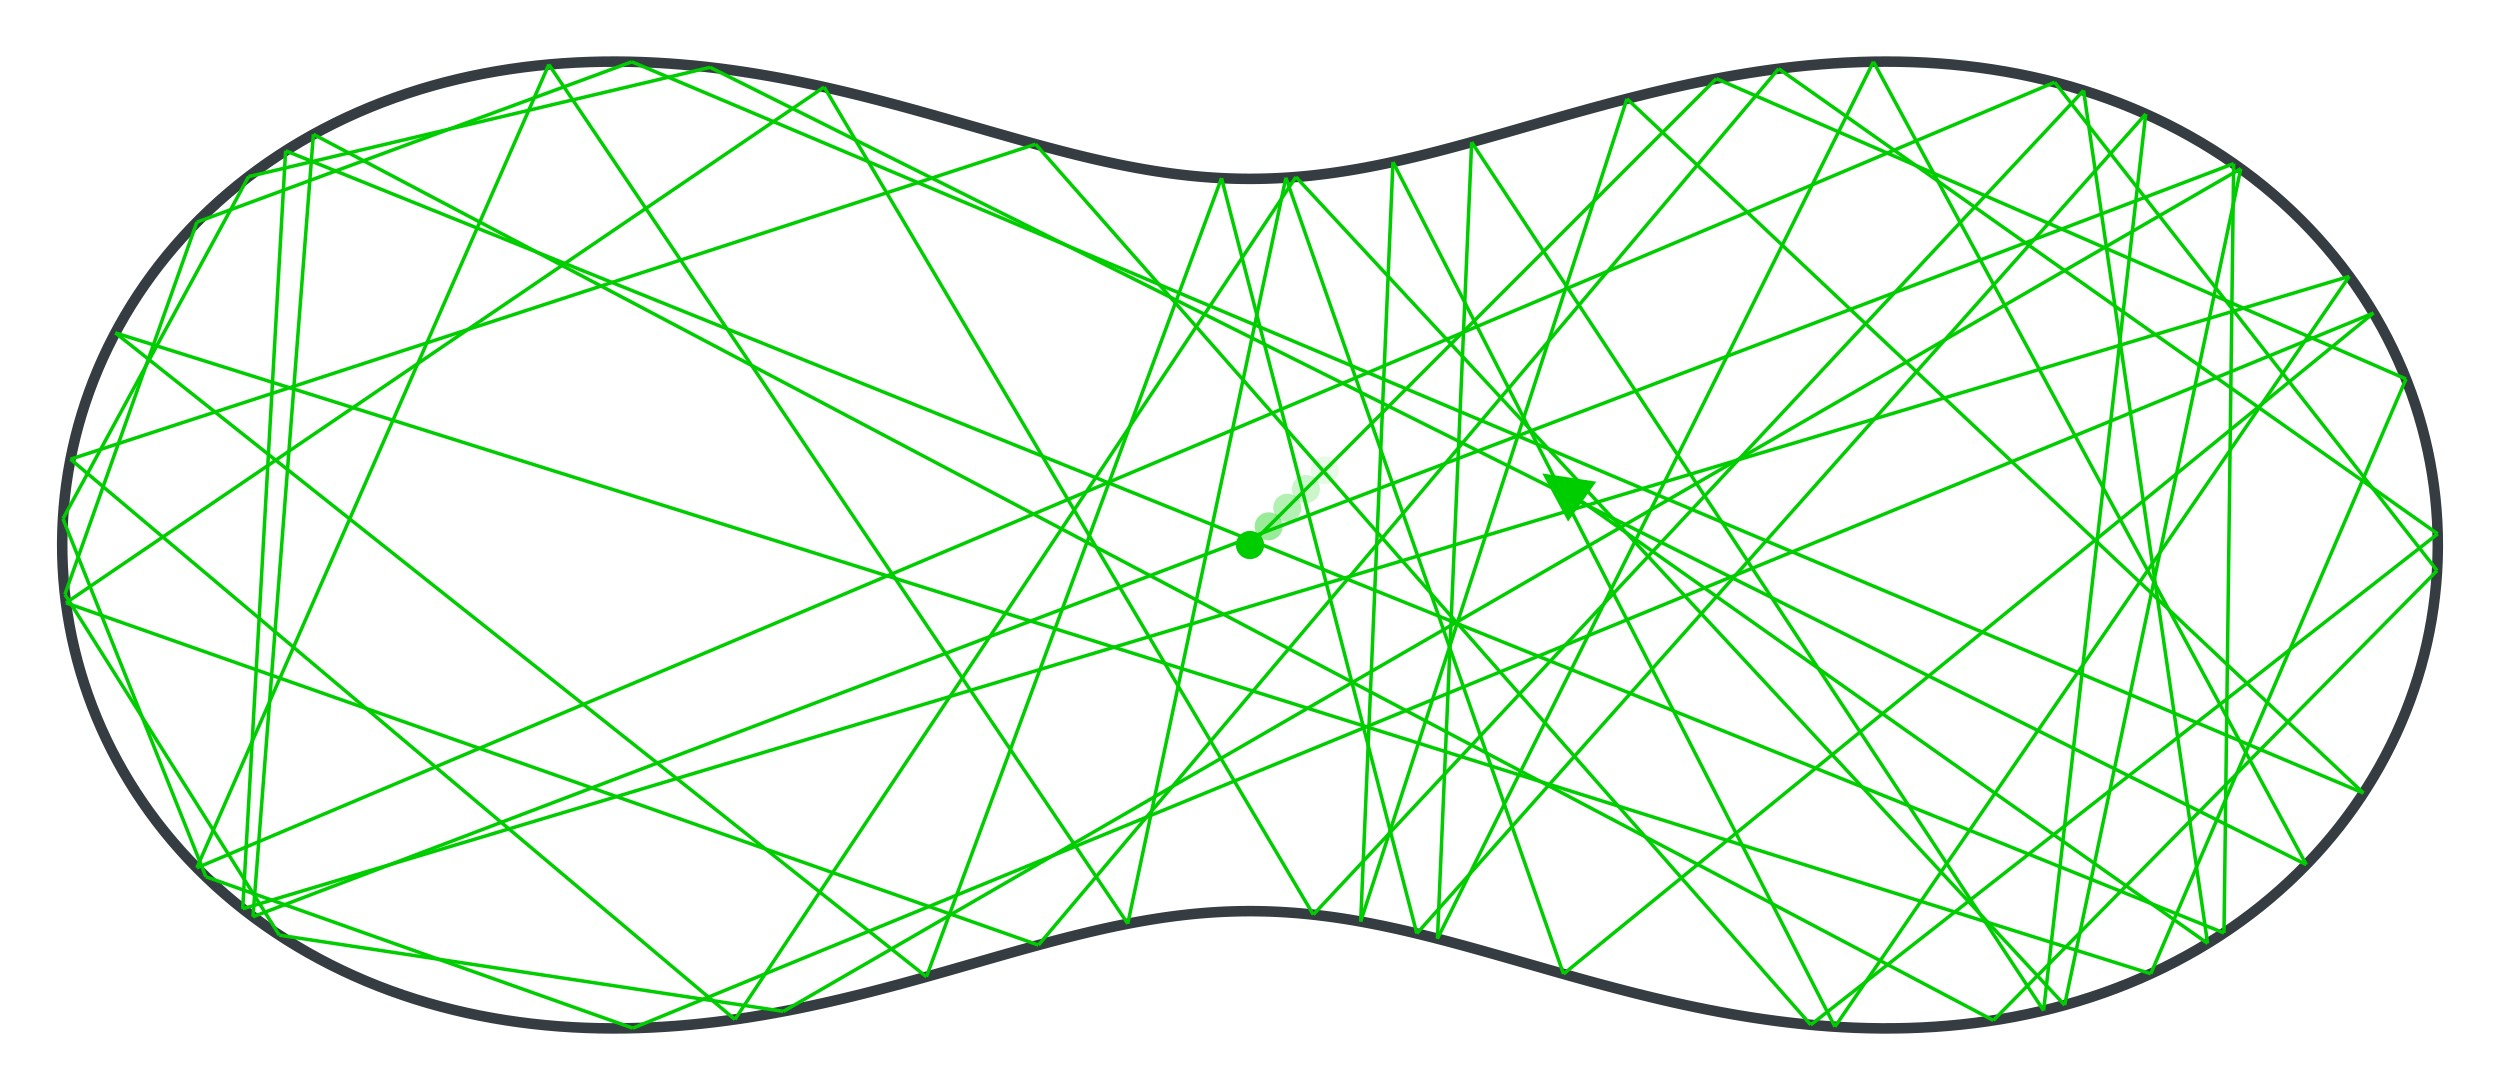
\includegraphics[scale=0.08,angle=0]{Cassini_true.jpeg}
    %\caption{Variabili $X_{n}$}
    \label{fig:oval}
  \end{subfigure}
    \noindent\\
  \begin{subfigure}[b]{0.4\textwidth}
  \centering
    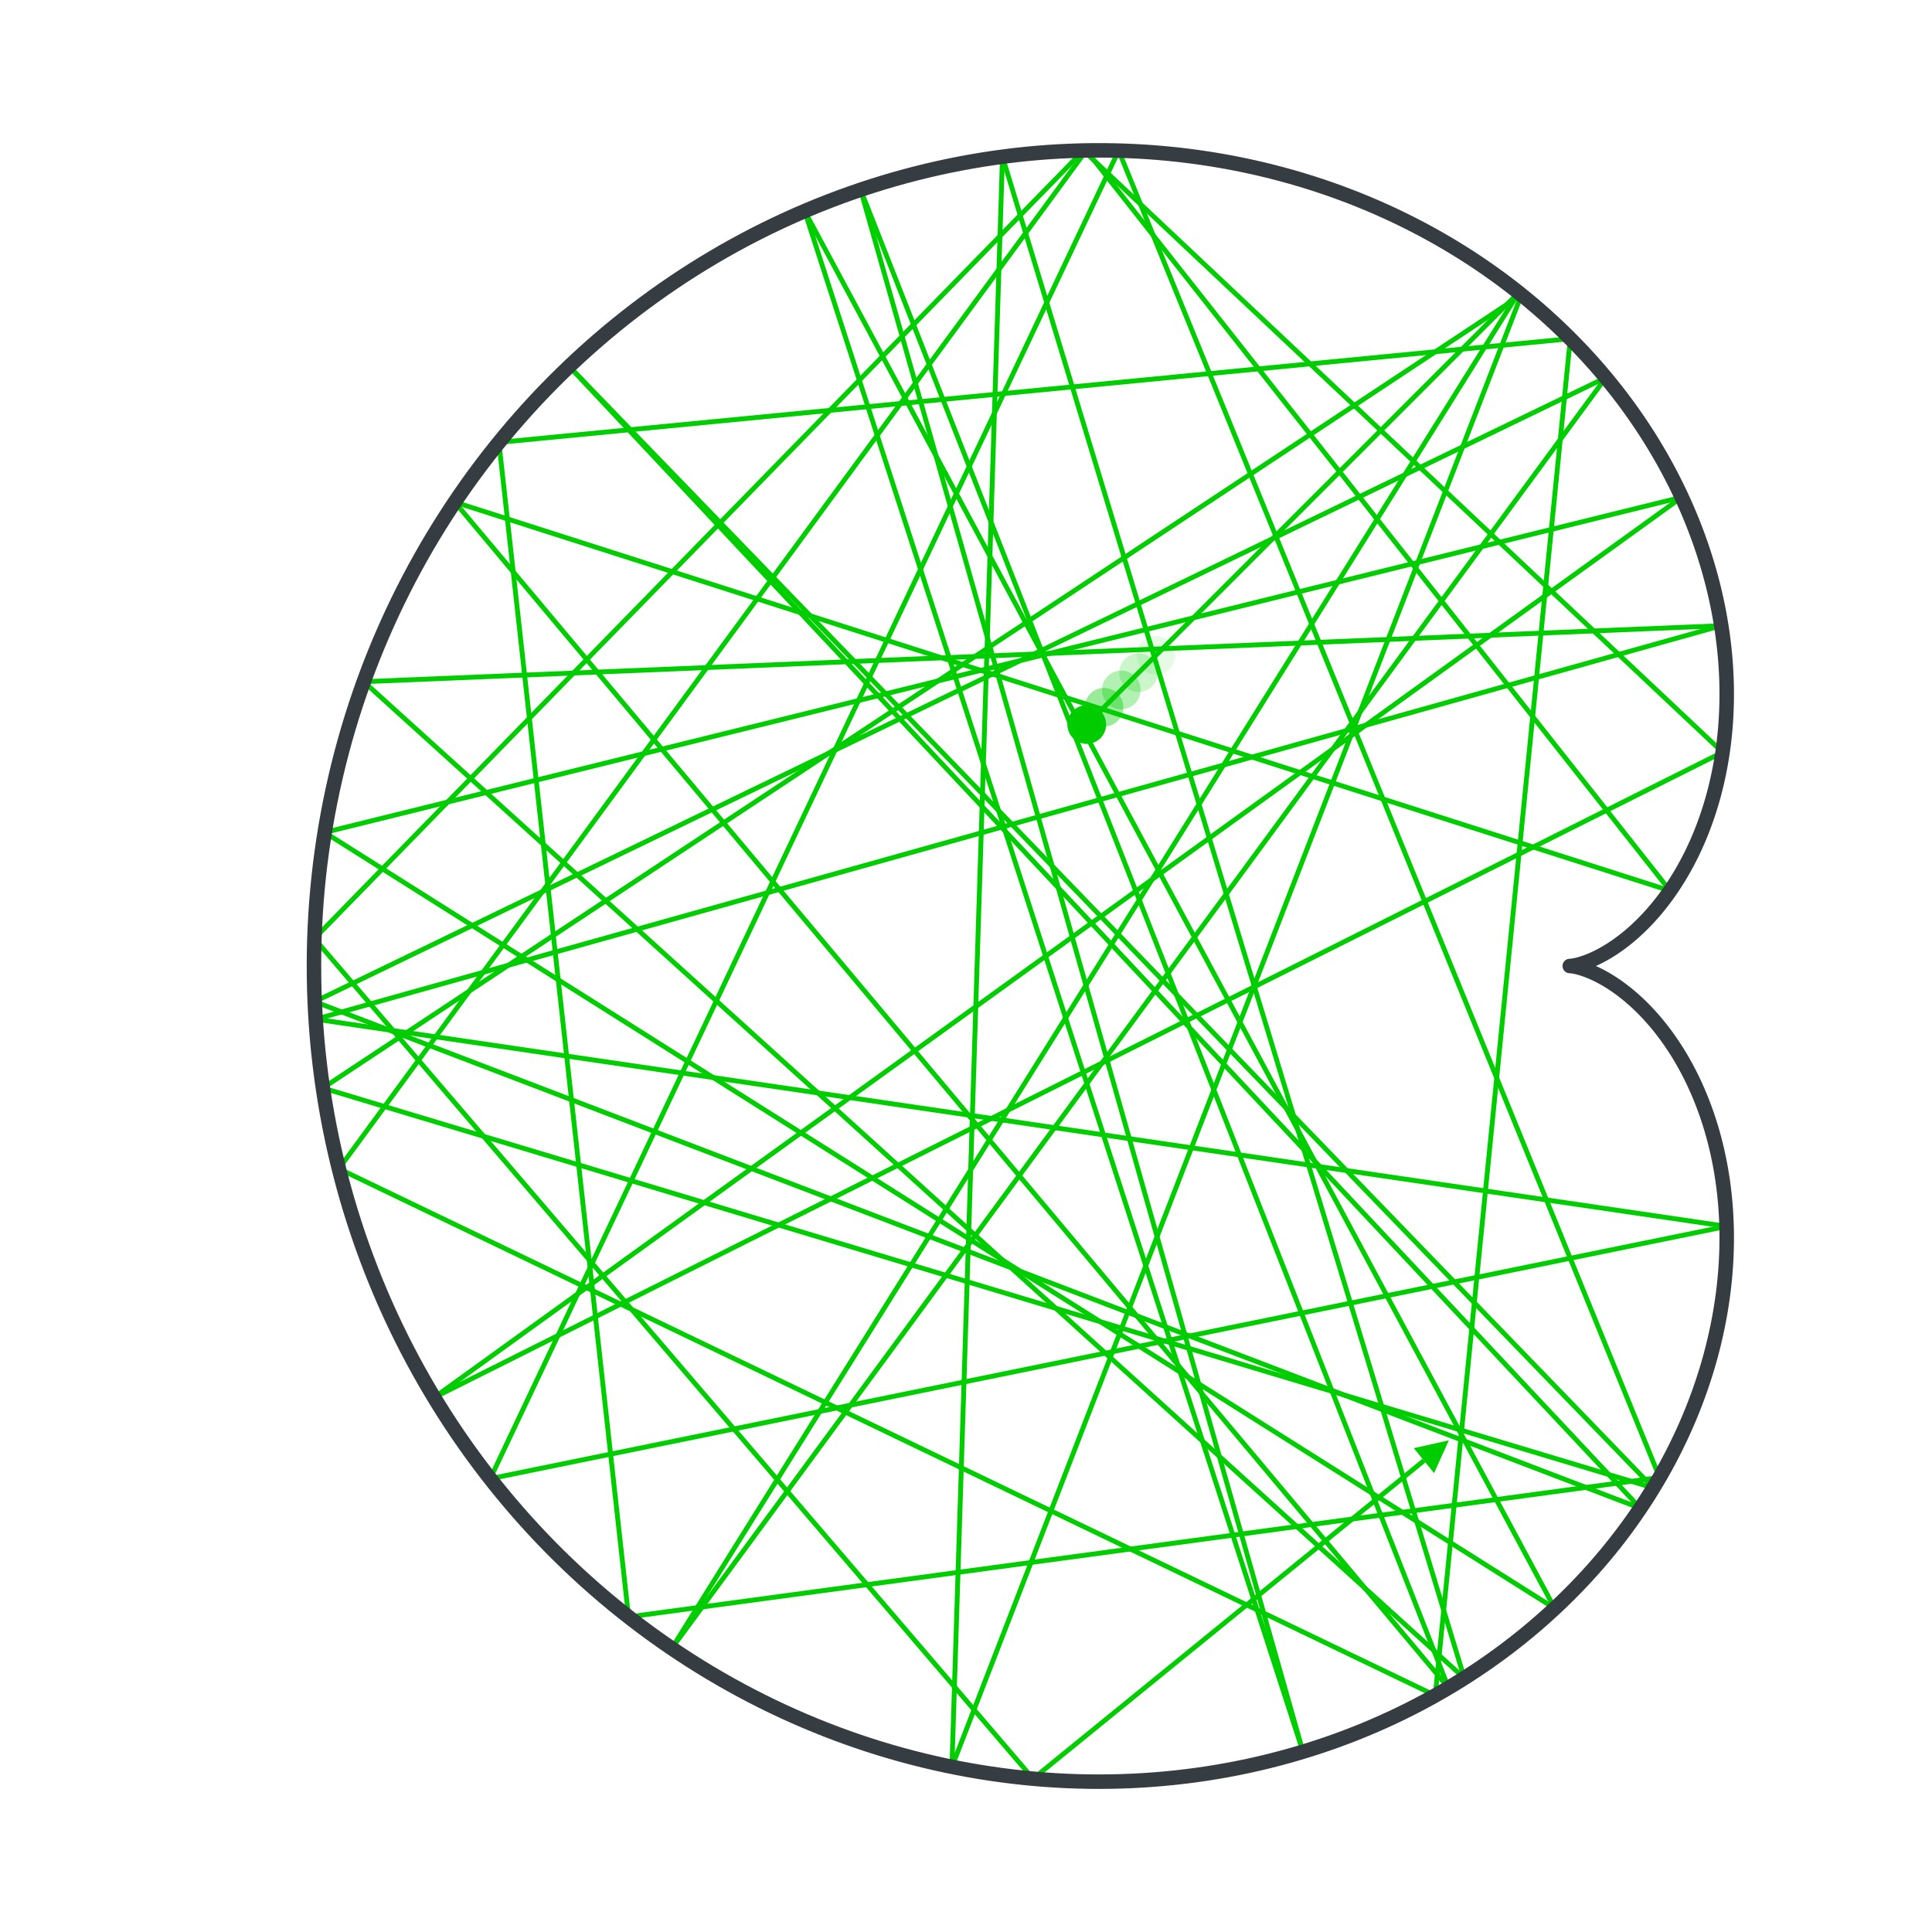
\includegraphics[scale=0.06,angle=0]{Cardioid.jpg}
    %\caption{Variabili $X_{n}$}
    \label{fig:cass}
  \end{subfigure}
  \noindent\\
  \decoRule
  \caption{Billiard trajectories in the Cassini's oval and Cardioid.}
  \label{fig:oval_card_orbits}
\end{figure}

As mentioned before, there are also \virg{billiards} induced by geodesic flow on a Riemannian manifold. The flow on the modular surface is a good example of this case (see chapter \ref{Chapter1}).

\begin{nese}[Modular surface]
It can be shown that on every Riemannian manifold with negative curvature, the geodesic flow $\Phi_{t}$ is ergodic (see Hopf theorem \ref{teo:Hopf_theorem}). The geodesic flow on the unit tangent space of the modular surface $\PSL_{2}\Z\setminus\Hilb$ (\ref{subsec:hyp_surfc}) is hence ergodic.
\end{nese}


\begin{figure}[H]
\centering
  %
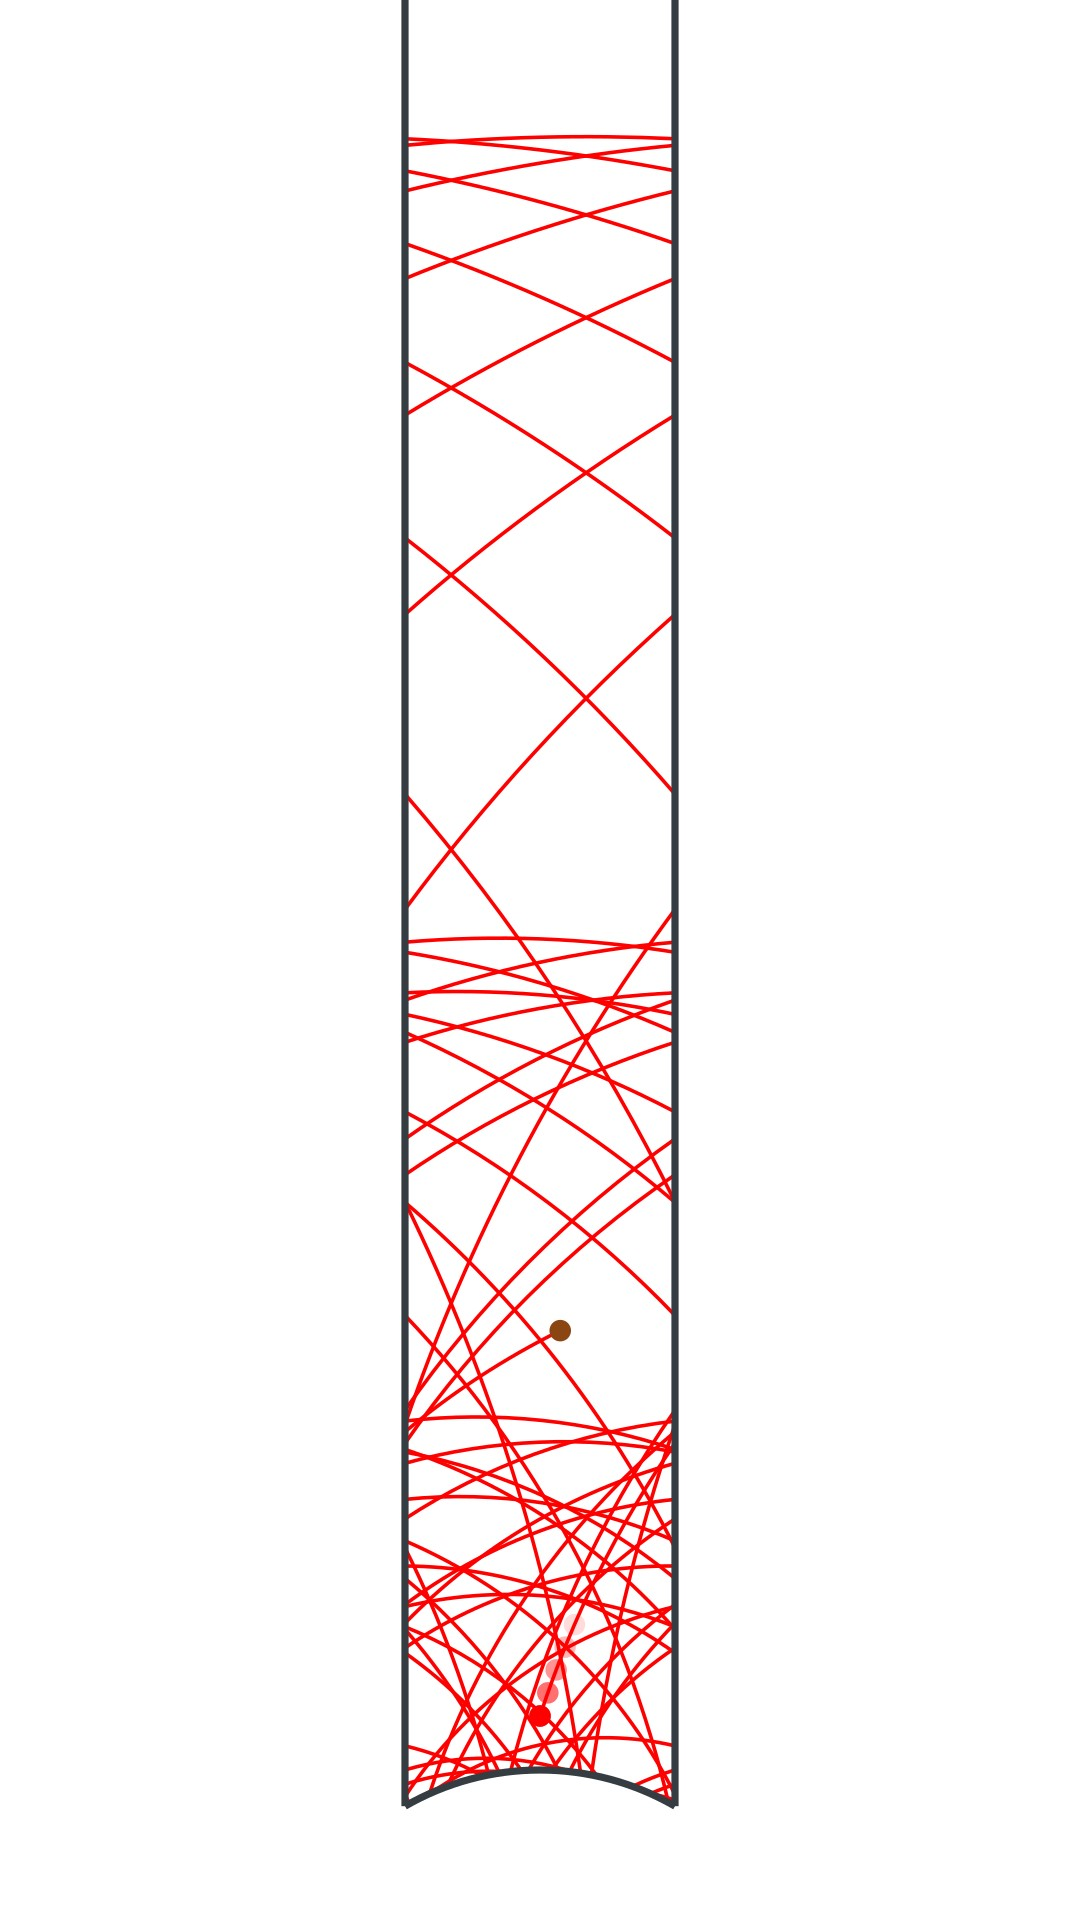
\includegraphics[scale=0.12,angle=0]{modular_good.jpg}
  \noindent\\
  \decoRule
  \caption{Ergodic orbit on the modular surface.}
  \label{fig:oval_card_orbits}
\end{figure}





\section{From classical to quantum billiards}


\subsection{Unique ergodicity}


Before introducing the \virg{quantum} definition of ergodicity, we recall the definition of unique ergodicity. In general, we give the following definition.

\begin{defin}
\label{def:unique_ergodic}
An ergodic metric system $(X,R,\mu_{L})$, where $\mu_{L}$ the standard Liouville measure, is called \emph{uniquely ergodic} if $\mu_{L}$ is the only finite borel measure, invariant with respect to $R$.
\end{defin}

The definition in the continuos case is essentially the same. The two condition of
\begin{compactenum}
\item finiteness,
\item uniqueness,
\end{compactenum}
are very strong. To this, consider a metric space $(X,R,\mu_{L})$, and a point $x\in X$ which is periodic. The dirac measure concentrated on points of the finite orbit of $x$ is preserved, but it is not the Liouville measure. We can appreciate the crucial point played by periodic orbits, in this framework.

\subsection{Quantum regime}

In quantum regime, billiards are described by wavefunctions $\psi_{n}$ whose time-evolution are ruled by the \emph{Schr{\"o}dinger equation}
\[
\imi\hbar\frac{\partial}{\partial t}\psi_{n}(x,t)=-\frac{\hbar^{2}}{2m}\Lapl\psi_{n}(x,t),
\]
where $\Lapl$ depends on the metric considered, with Dirichlet boundary conditions in the planar euclidian case. Moreover $\psi_{n}\in L^{2}(\Omega),\hbar$ is Planck's constant and $m$ is the mass of the particle. From quantum mechanics the generic time dependent solution is the superposition of time dependent solution of the form $\psi_{n}(x,t)=\exp(-\imi t E_{n}/\hbar)\vphi_{n}(x)$, where $E_{n}$ are quantum energy levels and $\vphi_{n}$ are eigenfunctions of the equation 
\[
-\frac{\hbar^{2}}{2m}\Lapl\vphi =E_{n}\vphi.
\]
So, the \virg{quantum-mechanical} evolution of the billiard is linked to the eigenvalue problem $-\Lapl\vphi_{n}=\lambda_{n}\vphi_{n}$, where $\lambda_{n}=2mE_{n}/\hbar^{2}$. Semiclassical analysis, among other things, deals with find a correspondence between classical motion and the quantum approach. Indeed, the starting question is: how is it possible to translate the concept of ergodicity in this quantum framework, from the classical one?

The feature of ergodicity that it is considered is equidistribution of orbits. We will know pause rigorous mathematical exposition for a brief informal introduction to the subject.\\
Let's consider the eigenfunction $\vphi_{j}$ corrispondent to the eigenvalue $\lambda_{j}$. Considering the absolute square $\abs{\vphi_{j}}^{2}$, we get a probability distribution on our billiard $\Omega$ or manifold $M$. There is a \emph{standard} way to lift this probability measure to the unit tangent space, using Wigner measures (see \ref{def:Wigner_measure} for further informations). Roughly speaking, for a smooth function $f\colon T^{1}\Omega=\Omega\times S^{1}$   on the unit tangent space, we can define the Wigner measure $\mu_{\vphi}$, and hence the integral $\mu_{\vphi}(f)$, induced by the eigenfunction $\vphi$ as 
\[
\mu_{\vphi}(f)\coloneqq\pscl{\Op(f)\vphi}{\vphi}_{L^{2}}
\]
where, if $\hat{\psi}$ is the Fourier transform of $\psi$,
\[
\Op(f)\psi(x)\coloneqq\int_{\R^{2}}\e^{2\pi\imi(x\cdot\xi)}\hat{\psi}(\xi)f\left(x,\frac{\xi}{\norm{\xi}}\right)\dd\xi.
\]
In particular, $\Op$ operator is a \emph{pseudo-differential operator} induced by function $f$. In \ref{subsec:how_to_quant} it is explained that this is only one possibilites, as there are other similar way to produce the operator $\Op$, e.g. another one is \emph{Weyl quantization}.\\
A \virg{natural way} to rewrite the idea \virg{a.e. orbit distributes itself uniformly} in the quantistic case is to formulate the following.

\begin{defin}
\label{def:roughly_qe_def}
A dynamical metric system is quantum ergodic if it does exist a subsequence of eigenvalues $\lambda_{k}$ for the Laplacian $\Lapl$ of density one, such that $\mu_{k}(=\mu_{\vphi_{\lambda_{k}}})$ converges weakly to the Liouville measure $\mu$.
\end{defin}

As will see in section \ref{sec:que_intro}, any weak limit for measures $\mu_{j}$ is called \emph{quantum limit}. Then, the concept of \emph{unique quantum ergodicity} is translated as follows.

\begin{defin}
\label{def:roughly_que_def}
A quantum system is unique ergodic if the only possible quantum limit is the standard Liouville measure.
\end{defin}

A case of particular interest is the one of hyperbolic surfaces $X$, with the Laplacian operator adapted to the hyperbolic metric \ref{sec:hyp_plane}. In this case, the Liouville measure is given by $\mu=\frac{1}{2\pi\lambda(X)}$, where $\lambda(X)$ is the hyperbolic measure of the hyperbolic surface $X$. The reason behind this interest is the following.

\begin{nteo}[Hopf]
\label{teo:Hopf_theorem}
Let $X$ be an hyperbolic surface. Then the geodesic flow on $T^{1}X$ is ergodic.
\end{nteo} 


\subsection{Some insights about \QUE}


A main result regarding \QE theory is due to Schnirelman,
Zelditch and Colin de Verdière, as we will see in chapter \ref{Chapter3}. Its statement is roughly the following.

\begin{nteo}
\label{teo:preview_quantum_ergod_theorem}
If a classical system is ergodic, then the corrisponding quantum system is \QE.
\end{nteo}

In particular, this gives us that Bunimovich stadium billiard $\BS$ and Barnett's billiard $\BarS$ are \QE. Moreover, all for all hyperbolic surface, \QE holds. So, the following question, made by Colin de Verdiére, was:
\begin{center}
What are the possible quantum limits?
\end{center}
Driven by theoretical considerations and numerical simulations, Rudnick and Sarnak proposed, in 1993 \cite{RudSarn:conj}, the following conjecture.\\[2mm]
\noindent\boldsf{Conjecture}: \emph{For all hyperbolic surfaces, \QUE holds}.\\[2mm]
A great achievement, towards this problem, was reached in 2010, thanks to the groundbreaking result due to Lindenstrauss. His work (\cite{LindBourg:entropy},\cite{Linden:main_art}) earned him the Fields Medal.

\begin{teo}[Lindenstrauss 2006, Soundarajan 2010]
\QUE holds for every arithmetic hyperbolic surface. 
\end{teo} 

Without goind in details about what an arithmetic hyperbolic surface is, it is sufficient to know that these surfaces arise from arithmetic methods. So, Lindenstrauss used this information to impose more symmetry on Laplacian eigenfunctions, via \emph{Hecke operators}, which are genuinely arithmetic tools.\\
On the other hand, another important result about \QUE led to the opposite side of the conjecture, in the euclidian case. In fact, in the same year (2010) Hassell proved that \QUE doesn't hold for Bunimovich stadium (\cite{Hass:billiards_not}), as some \virg{bouncing back and forth} eigenstates are still present in the high-energy limit. For more details, see chapter \ref{Chapter3}.


\section{The classic-quantum correspondence}

We have outlined the main themes of this thesis, so maybe it is a good time to recall what our aim is.\\
We are interested in understanding how the ergodicityof the geodesic flow does determin the distribution of high-eigenvalue Laplacian eigenfunctions. We recall some informations from appendix \ref{AppendixA}.\\

On any classical system on a Riemannian manifold $(M,g)$, the geodesic flow is given by the Hamiltonian vector field $X_{H}$ generated by the Hamiltonian function $H\colon M\to\R$. Integrating the Hamiltonian vector field $X_{H}$ generates a one parameter family of integral curves. These curves represent the geodesic flow and so we can define $\Phi^{t}\colon M\to M$ which defines the time evolution of a point on the manifold $M$ along this flow. In this context, the manifold $M$ is the configuration space, while the cotangent bundle $T^{\ast}M$ of couples $(q,p)$ of position and momentum is the phase space.\\
We can consider the energy level sets $\Sigma_{c}\coloneqq H^{-1}(c)$, which carry a natural flow-invariant measure, called \emph{Liouville measure}. It can be charaterized not only by the invariance through the geodesic flow, but also in the following way.

\begin{defin}
\label{def:Liouville_measure}
The Liouville measure $\mu_{L}^{c}$ is the flow-invariant volume-form on any \virg{energy-shell} $\Sigma_{c}$ of a Hamiltonian system. In particular, for $c\in [a,b]$, $\mu_{L}^{c}$ is characterized by the formula
\[
\iint_{H^{-1}[a,b]}f\dd x\dd p=\int_{a}^{b}\int_{\Sigma_{c}}f \dd\mu_{L}^{c}\dd c,
\]
for a smooth function $f\colon T^{\ast}M\to\R$.
\end{defin}

Now, if $(M,g)$ is a compact manifold with negative curvature, Hopf theorem \ref{teo:Hopf_theorem} assure us that the geodesic flow is ergodic, with respect to Liouville measure. In particular, we will show this in section \ref{sec:hyp_dynam}, in the case of hyperbolic surfaces generated by Fuchsian groups. The corrisponding quantum dynamics is the unitary flow generated by Laplace operator, as a generic time evolution is given by superposition of eigenfunctions $-\Lapl\psi=\lambda_{n}\psi$. At this level, we can \virg{see} that, in some way, the ergodic geodesic flow influences the spectral aspect of the Laplacian, making its eigenfunctions equidistributed.\\

Having this in mind, in our humble opinion, it seems appropriate to pointing out some important themes for this thesis. These will be useful to keep in mind in chapter \ref{Chapter3}.

\begin{compactitem}
\item Intuition behind the semiclassical limit: even if, numerically, we can take the \emph{semiclassical limit} $\hbar\to0$, we need the energies to be bounded. So, in semiclassical regime, we aspect that the asymptotic behaviour of quantum objects corrispond to the classical one; 
\item The technical aspects of semiclassical analysis: Fourier transform enables us to relate position and momentum variables. So, as semiclassical limit relies on a global rescaling, we will a sort of semiclassical Fourier transform, hence classical Fourier transform theory will be useful.
\item Interaction between order and disorder, from simple cases: as it can be seen, lots of the results and problem of this theory is drawn by visualization and numerical simulations; even if starting examples are very simple, the theory behind it isn't and this framework is a good example of the dichotomy between classical structure and quantum randomness:\\[2mm]
\textit{The \virg{dichotomy between structure(order) and randomness} seems to apply in circumstances
in which one is considering a high-dimensional class of objects$\ldots$ one needs tools such as algebra and geometry to understand the structured component, one needs tools
such as analysis and probability to understand the pseudorandom component, and one needs tools such as decompositions, algorithms, and evolution equations to separate the structure from the pseudorandomness.}\\[2mm]
\hspace*{10cm}\textsl{Terrence Tao}, \cite{tao:site_simons_lec}
\end{compactitem}

















